\chapter{Evaluation}\label{chap:evaluation}
	In this part of this thesis the models and methods outlined in the project will be evaluated. As outlined in the previous chapter, an experimentation interface was built to parametrize the assembly of the dataset and use different learning machines for each parameterization. First, the data will be extracted from the xml-files and stored with the pipeline in npy-files as matrix form. These will be used for each experiment set with different parametrization, i.e. frequency and maximum number of frames allowed. These parametrization can be tweaked to evaluate the used methods in this thesis and gauge the performance enhancement through using them.\newline
	This chapter with be divided into two main parts. Firstly, the vanilla learning machines that build a one-to-one relationship will be evaluated. Next, recurrent neural models will be examined and evaluated. This evaluation is by no mean an exhaustive use of the experimentation interface and only provide an insight to each use case, where a significant increase of performance was observed. This is mainly due to the complexity of training recurrent neural networks, which in average takes between three hours for four epochs.\newline
	As for the training, all the results were obtained by using the Adam optimizer and an adaptive learning rate that is reduced by an order of magnitude at the end of each epoch and an initial value of 0.0001. In addition to that, each model was trained in a total amount of 9 epochs.\newline
	\begin{figure}[H]
		\centering
		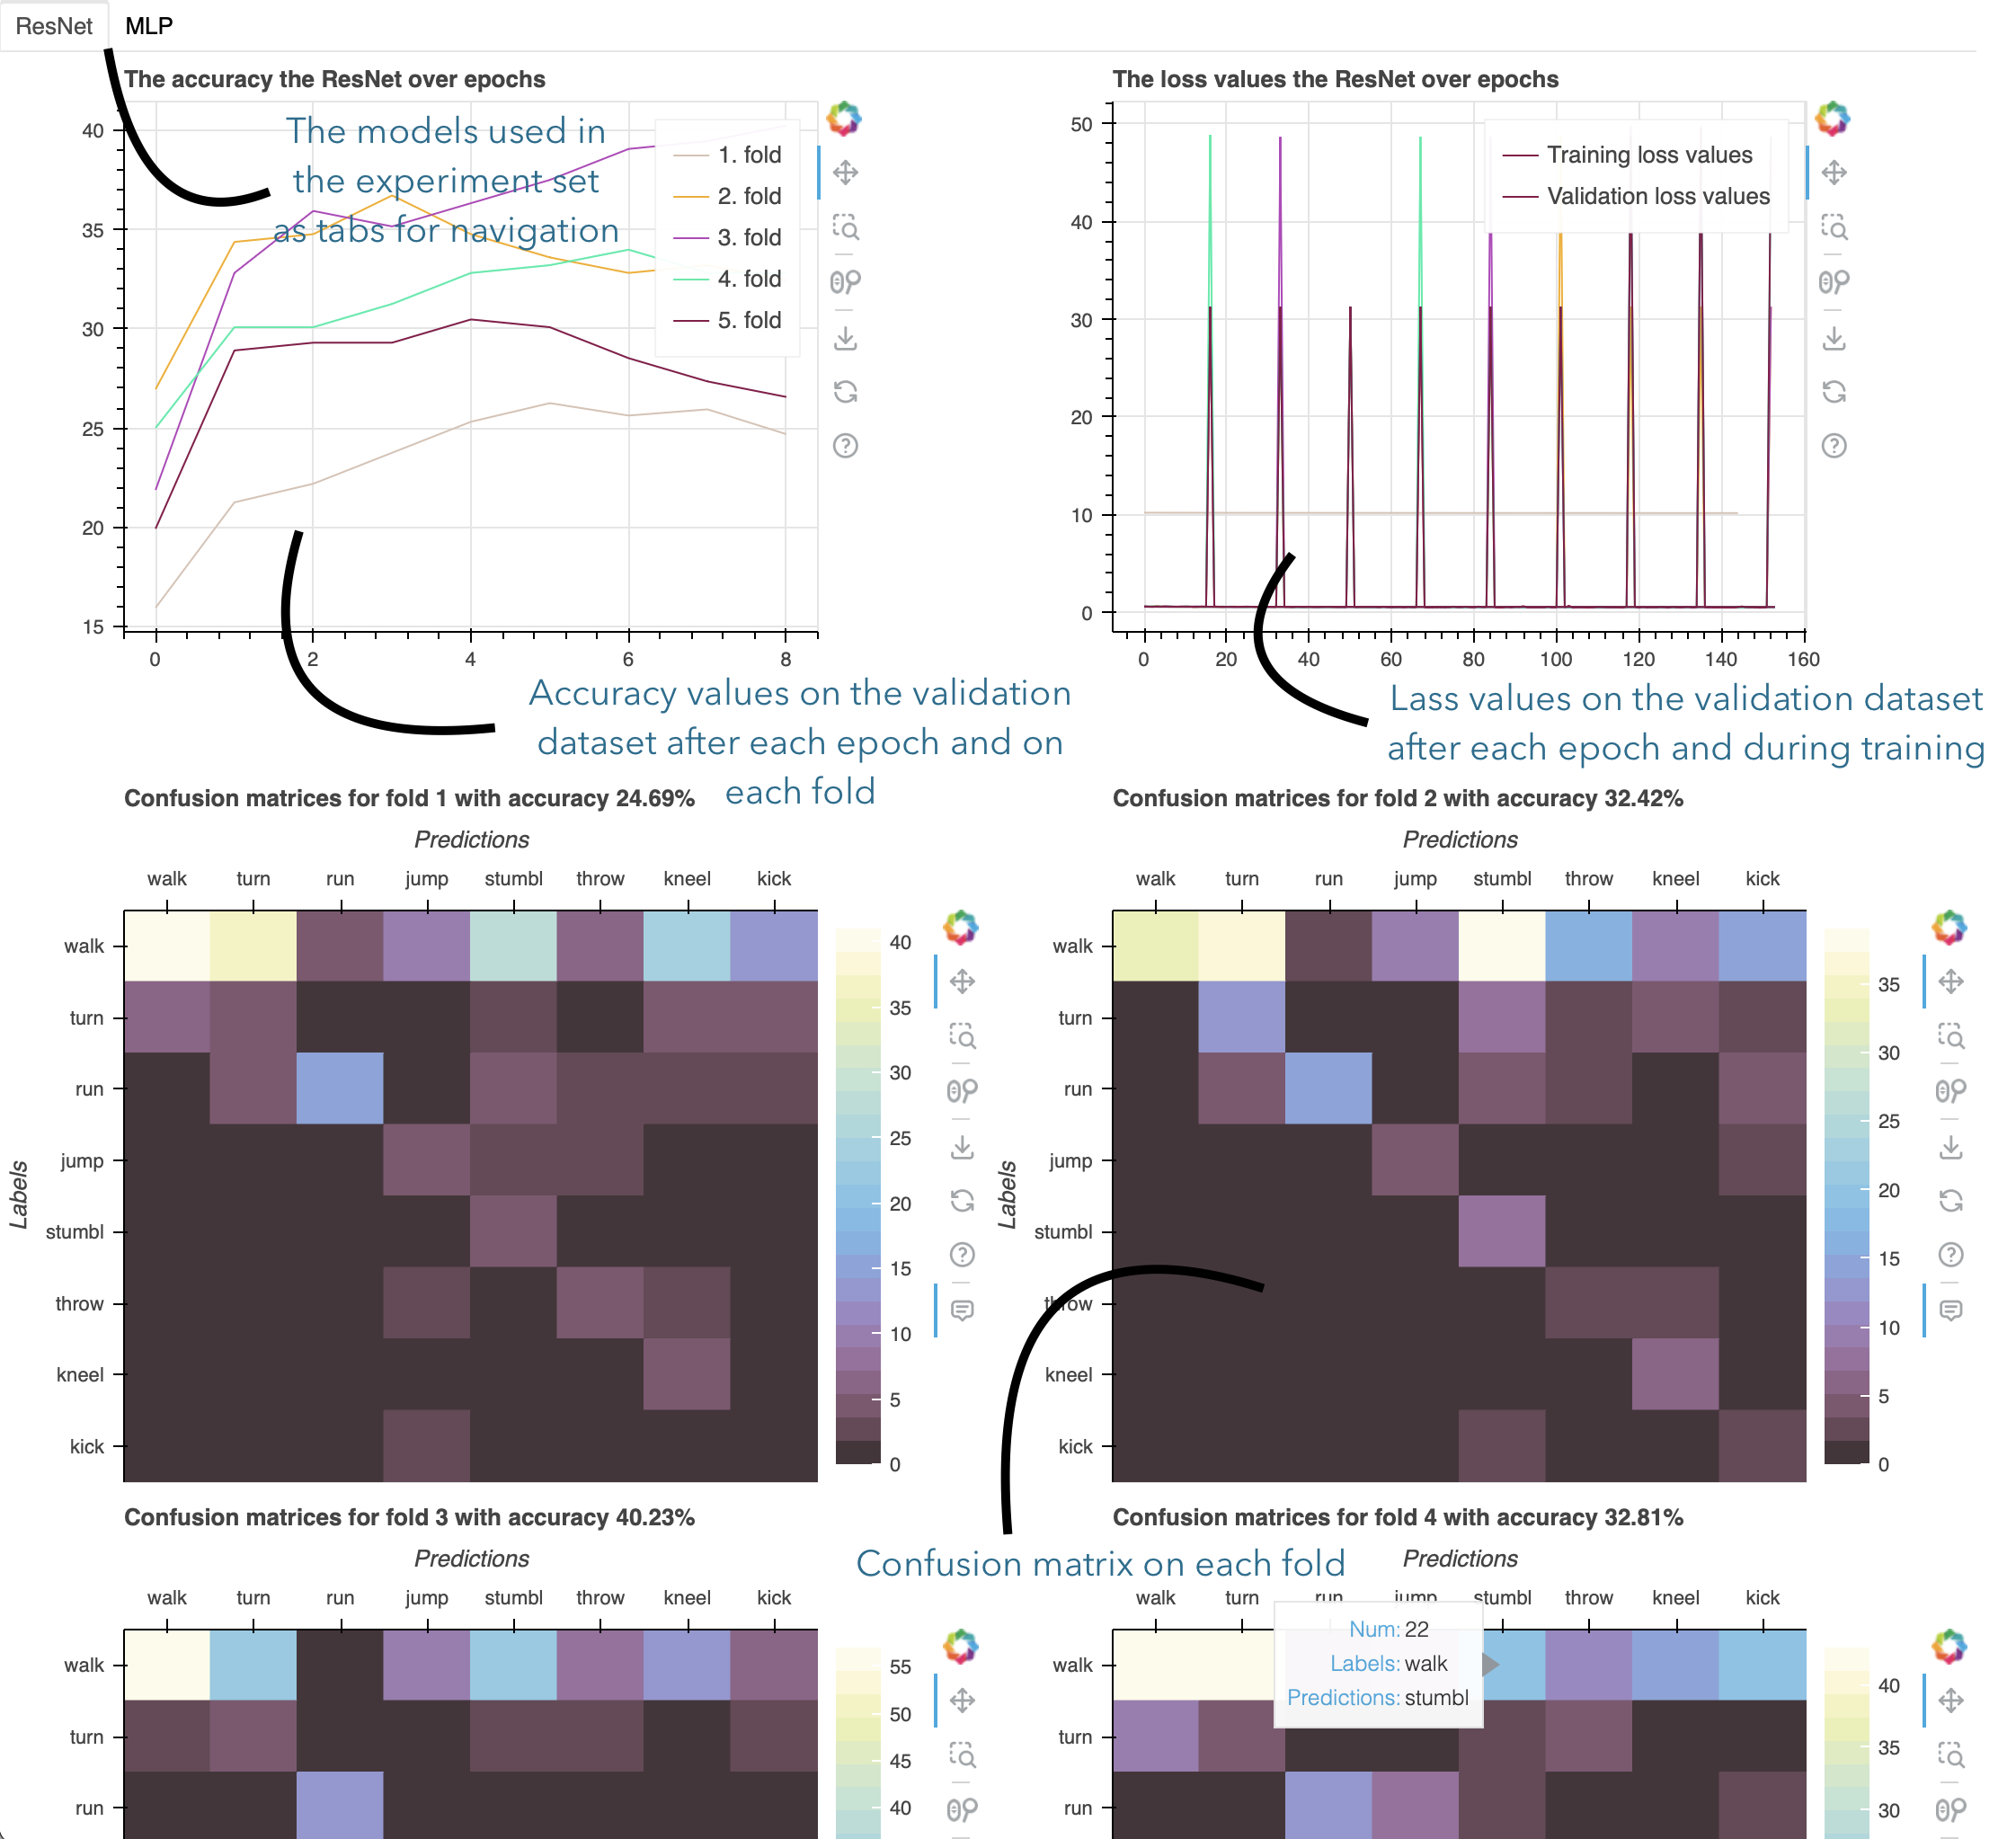
\includegraphics[width=\textwidth]{img/the-interface-of-the-visualisation-of-the-results-for-each-experiment-set.png}
		\caption{The interface of the visualisation of the results for each experiment set}
		\label{fig:vis_example}
	\end{figure}
	In fig \ref{fig:vis_example} the interface of the visualisation of the results for each fold is shown, where tabs are used to separate the results of each experiment in the experiment set. To distinguish between the visualizations of each experiment set the name of the corresponding file can be used, with the following syntax the general parameters of the experiment files is \textit{Experiment\_<num\_features>\_<frequency>\_['n' if normalized else '']['o' if oversapling\_used else '']}, where \textit{num\_features} reflect if:
	\begin{itemize}
		\item 6 then the only the root information has been used in the experiment set,
		\item with 44 the position of each joint has been used, 
		\item and 50 all the data extracted from the xml-files was assembled in the dataset.
	\end{itemize}
	The files and the results of each experiment documented can be found in the folder \textit{plots} and creating a new experiment involves only creating a new \textit{Experiment.json} file and the predefined stems in the file \textit{labels.json}. However, due to the sheer amount of data in these files only the results will be discussed in the next sections, and the visualization files can be used as a reference. Nevertheless, the user can still create and run his/her own experiment sets with different parameterisations of the datasets and hyper parameters for recurrent neural networks. For this purpose some examples can be found in the \textit{Experiments} folders and can be used as templates.
	\section{One-to-one learning machines}\label{subsec:eva_one2one} 
		For this section the following learning machines will be used:
		\begin{itemize}
			\item MLP with the following layers and using the \textit{ReLU} as an activation function between each layer;
				\begin{itemize}
					\item input layer that take the flattened motion matrix and has a size of number of frames multiplied by the number of features.
					\item the first hidden layer with 1024 neurons.
					\item the second hidden layer with 2048 neurons.
					\item the output layer, that generate a probability distribution using \textit{softmax}.
				\end{itemize}
			\item CNN with the layers in the same order;
				\begin{itemize}
					\item 1d-Convolution with kernel size 3,
					\item a batch normalization layer to reduce overfitting as stated in \ref{subsec:dnn}, with 4 channels
					\item Next the activation function \textit{ReLU} is used,
					\item 1d-Convolution with kernel size 3
					\item the next Batch normalization layer with 8 channels,
					\item then the activation function \textit{ReLU},
					\item 1d-Convolution with kernel size 3
					\item the next Batch normalization layer with 16 channels,
					\item then the activation function \textit{ReLU},
					\item 1d-Convolution with kernel size 3
					\item the next Batch normalization layer with 32 channels,
					\item then the activation function \textit{ReLU},
					\item 1d-Convolution with kernel size 3
					\item the last batch normalization layer with 11 channels,
					\item then the activation function \textit{ReLU},
					\item lastly, an average pooling layer,
					\item and the preparation for the output layer with Flatten,
					\item the output layer, that generates a probability distribution using \textit{softmax}.
				\end{itemize}
			\item FCN has the same architecture as in the CNN but forgoes the batch normalization layers.
			\item ResNet is comprised of three ResNet-blocks as in \ref{fig:wang2017timeresnet} and each ResNet-Block has the following layers and the output of each block is summed with its input and forwarded to the next block;
				\begin{itemize}
					\item 1d-Convolution with kernel size 3,
					\item a batch normalization layer to reduce overfitting as stated in \ref{subsec:dnn}, with 4 channels
					\item Next the activation function \textit{ReLU} is used,
					\item 1d-Convolution with kernel size 3,
					\item the next Batch normalization layer,
					\item then the activation function \textit{ReLU},
					\item 1d-Convolution with kernel size 3,
					\item the last batch normalization layer,
					\item then the activation function \textit{ReLU},
				\end{itemize}
		\end{itemize}
		In summery, these model proved to be very resilient and without oversampling it performed very well in comparison to sequence modelling learning machines, which only performed well with oversampling, a good indication of overfitting. However, due to the use of the weighted loss function instances of the \textbf{walk} class were greatly misclassified in comparison to other models. The culprit here is the inter-class similarity, where the learning machines find it hard to find and learn good features for each class. In addition to that, the loss value for the validation sets plateaus after few epochs. This also the case for the loss values during the training, where after taking the first batches in the training set the loss values swing in a small interval and plateau after processing the first batch. This is clearly illustrated in fig \ref{fig:accuray_loss_one2one_models}.\newline
		Interestingly, using normalization for the informations about the joints proved to contra productive and looking closely into the data, it is clear that normalization would be unnecessary due to the nature of this information. Concordantly, these reflect the rotational position in rad of each joint on each rotation axis and are within the interval between 0 and 3.4. Nevertheless, using normalization for the in the data about the position of the root joint was very fruitful due to the fact that it reflect the real coordinated of the position of the root joint and must be normalized to remove unnecessary features in the data, i.e. the position of root joint according to a coordinated system.\newline
		As for oversampling, it can be clearly stated that the trained model are highly overfitted and using it leads to better accuracy overall but it can't be categorically determined that model are not generalizable.
		\begin{figure}[H]
			\centering
			\begin{subfigure}[b]{0.49\textwidth}
				\centering
				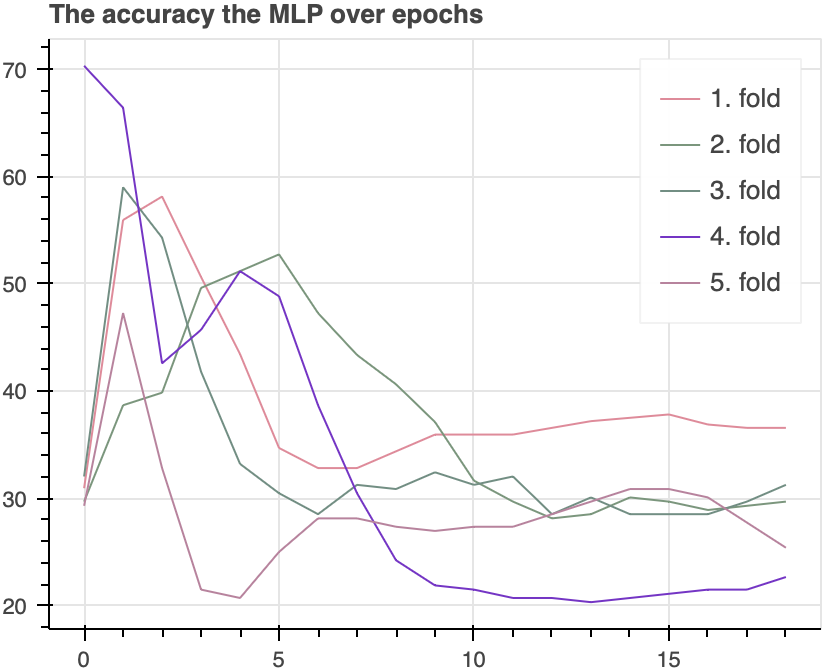
\includegraphics[width=\textwidth]{img/MLP_accuracy.png}
			\end{subfigure}
			\hfill
			\begin{subfigure}[b]{0.49\textwidth}
				\centering
				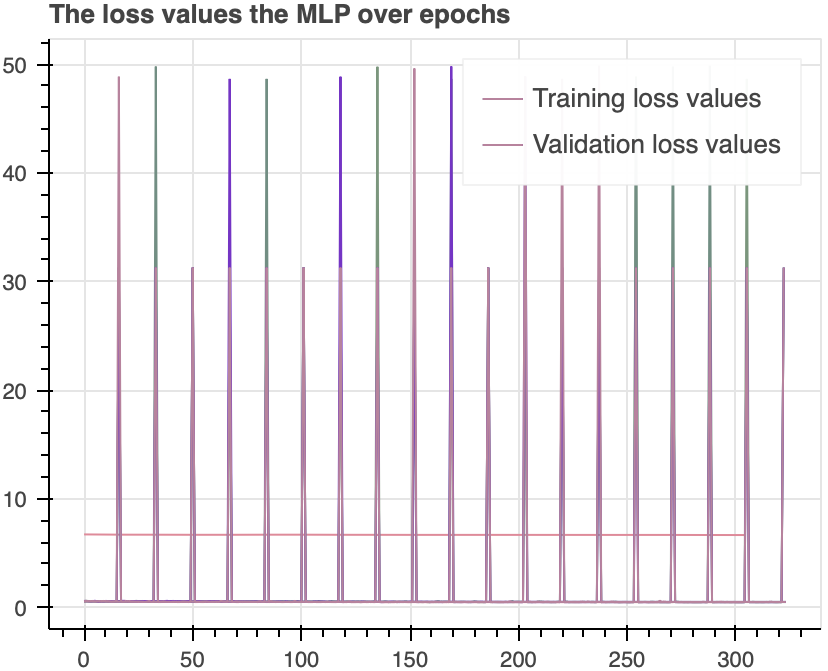
\includegraphics[width=\textwidth]{img/MLP_loss_values.png}
			\end{subfigure}
			\hfill
			\begin{subfigure}[b]{0.49\textwidth}
				\centering
				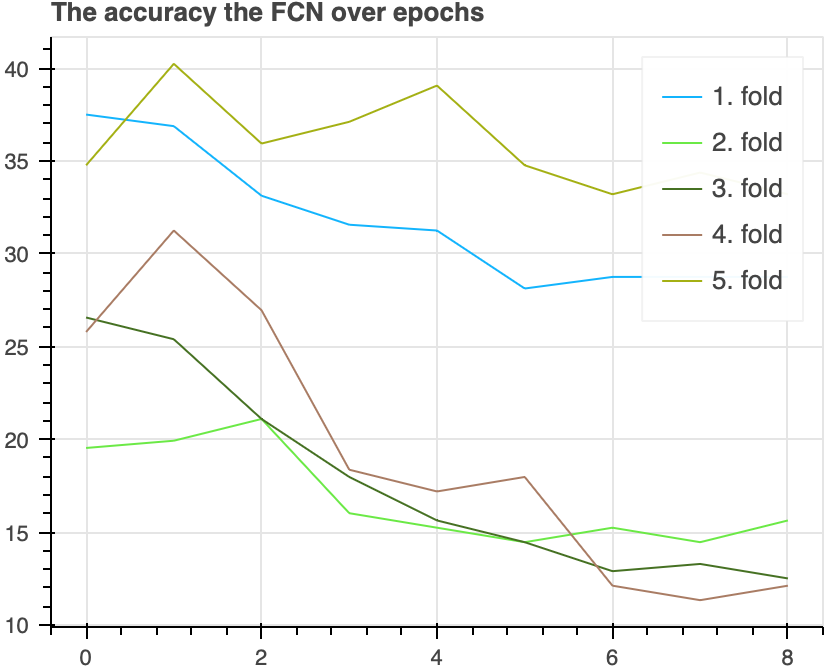
\includegraphics[width=\textwidth]{img/FCN-accuracy.png}
			\end{subfigure}
			\hfill
			\begin{subfigure}[b]{0.49\textwidth}
				\centering
				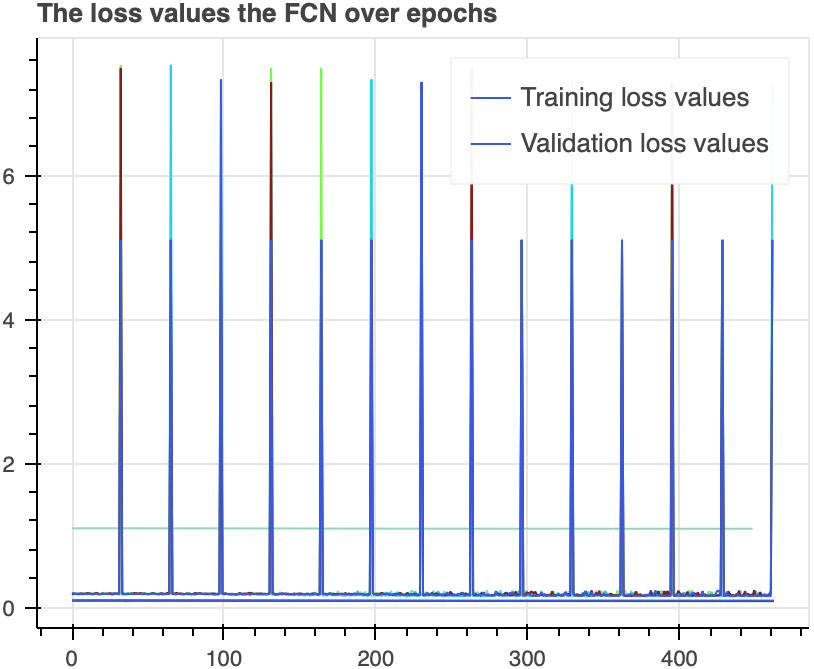
\includegraphics[width=\textwidth]{img/FCN-loss_values.png}
			\end{subfigure}
		\end{figure}
		\begin{figure}[H]\ContinuedFloat
			\begin{subfigure}[b]{0.49\textwidth}
				\centering
				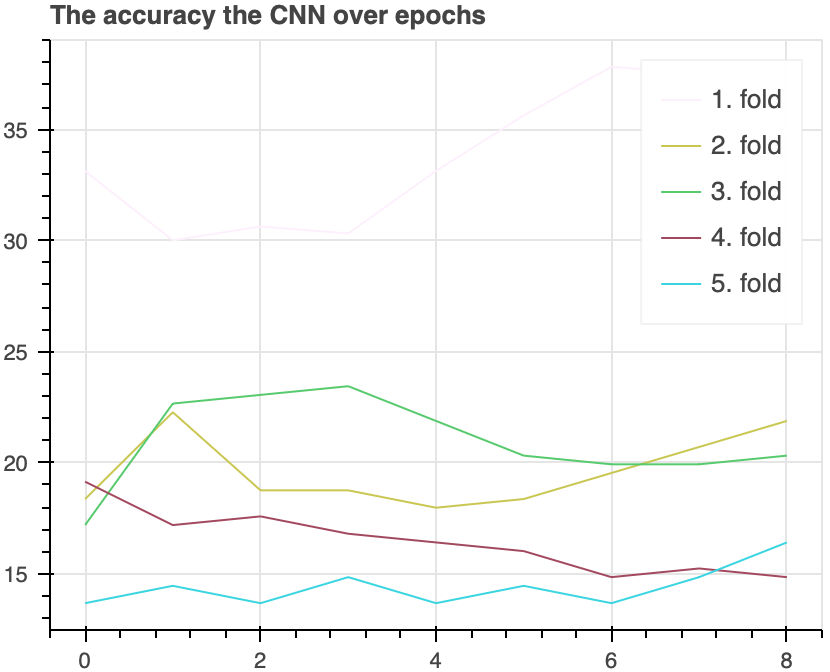
\includegraphics[width=\textwidth]{img/CNN_accuracy.png}
			\end{subfigure}
			\hfill
			\begin{subfigure}[b]{0.49\textwidth}
				\centering
				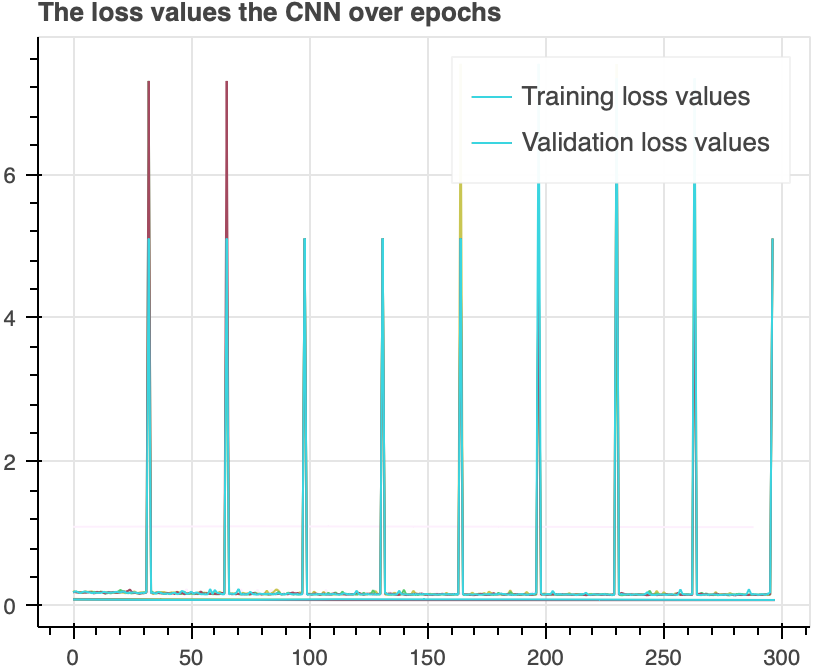
\includegraphics[width=\textwidth]{img/CNN_loss_values.png}
			\end{subfigure}
			\hfill
			\begin{subfigure}[b]{0.49\textwidth}
				\centering
				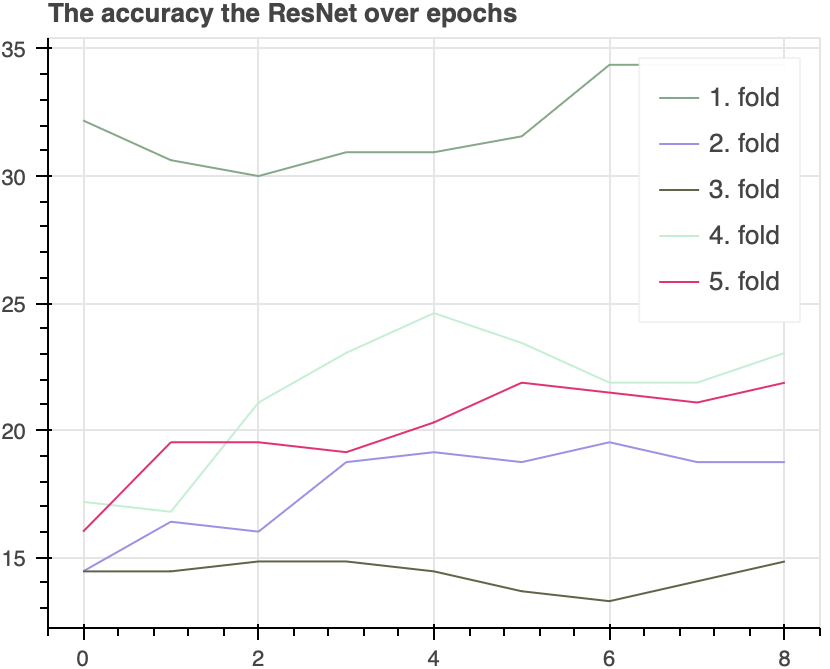
\includegraphics[width=\textwidth]{img/ResNet_accuracy.png}
			\end{subfigure}
			\hfill
			\begin{subfigure}[b]{0.49\textwidth}
				\centering
				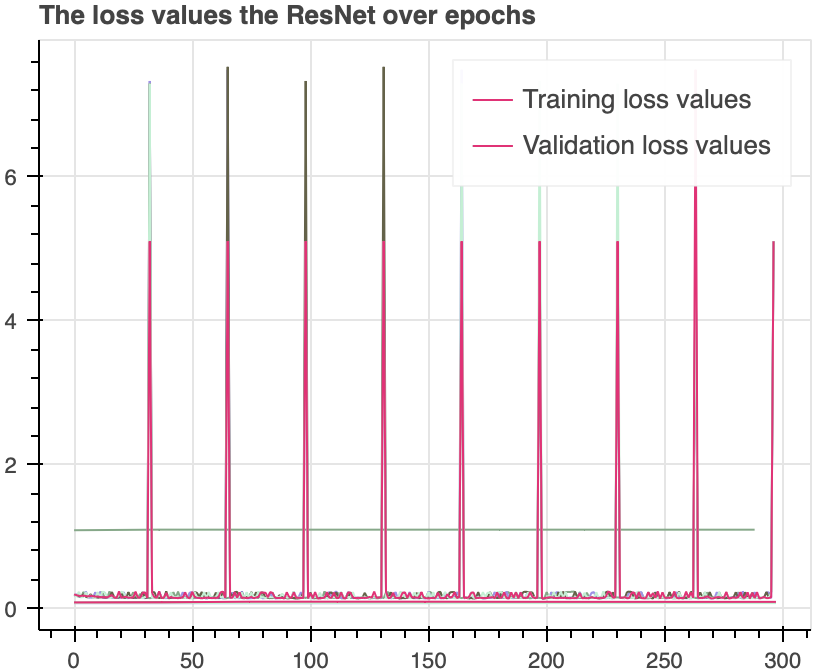
\includegraphics[width=\textwidth]{img/ResNet_loss_values.png}
			\end{subfigure}
			\caption{The accuracy rate and the loss values over the epochs and during the training of one-to-one models}
			\label{fig:accuray_loss_one2one_models}
		\end{figure}
		First, the data stored in xml-file was used without normalization or oversampling to see, if these offer any advantage and check in which case this might be detrimental to the overall performance of the trained learning machines. Taking different parameters into account can establish a relationship between good features and good representation of each class of motions.\newline
		By using only the available data for the root joint to train the models it can be said that the models performed very well with regard to the less represented classes. This is due to the fact, that a weighted version of the cross entropy loss was used, which penalizes the model more for a misclassification of a less represented class in comparison to a misclassification of the more dominant classes in the dataset. Moreover, it must be diligently noted that judging the models can't be done using the overall accuracy since it doesn't reflect the performance of the model as whole. Thus, in future expansion of this projects more metrics must be implemented to provide the experimenter more context to results obtained, even though the confusion matrix provide this in more a generalized sense. However, the use a non weighted version of cross entropy leads to models that classify all instances in the validation set as the most dominant class regardless of training time and makes its use for this task a net positive overall. Next, the results of training the models on the information about the joint positions show little improvement overall and the same can be stated for using all the available information in the dataset and more or less reflect the same about using only the data about the root joint.\newline
		Using normalization was beneficial for the overall case, but does contribute very little for using only the data about the joint position. However, using oversampling showed a very concerning trend against it, where the problem of inter-class similarity is further aggravated. Lastly, combining normalization and oversampling to combine the benefits of both approaches contributed more to the picture, but that was of very little significance with using the joint position in each frame. This makes the risk of overfitting more pertinent and would make the advice against using oversampling very reasonable.
		\begin{figure}[H]
			\centering
			\begin{subfigure}[b]{0.49\textwidth}
				\centering
				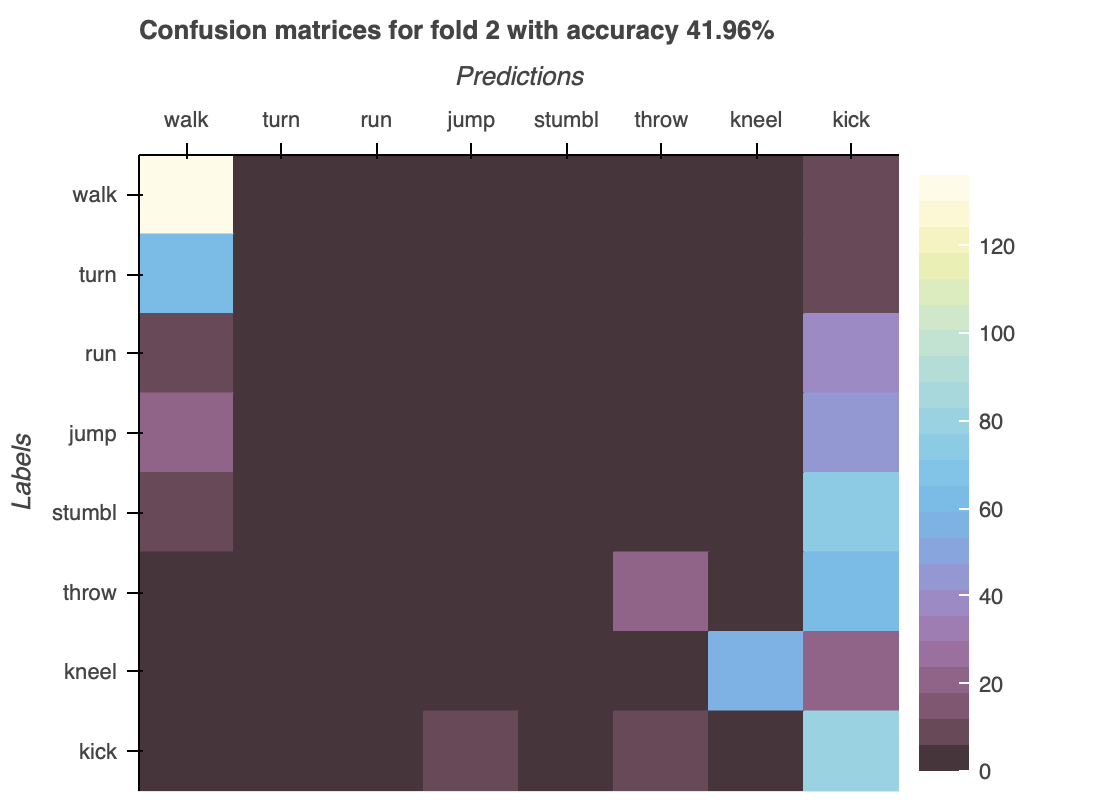
\includegraphics[width=\textwidth]{img/MLP-confusion_matrix.png}
				\caption{MLP}
			\end{subfigure}
			\hfill
			\begin{subfigure}[b]{0.49\textwidth}
				\centering
				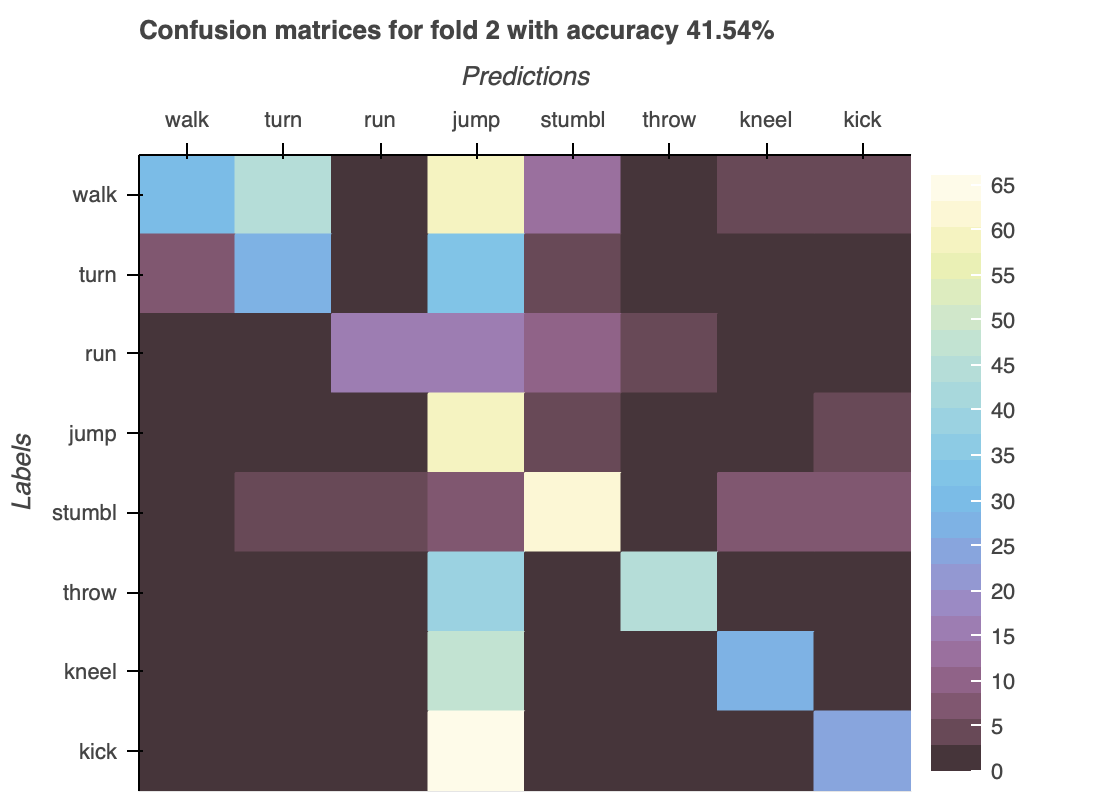
\includegraphics[width=\textwidth]{img/FCN-confusion_matrix.png}
				\caption{FCN}
			\end{subfigure}
		\end{figure}
		\begin{figure}[H]\ContinuedFloat
			\begin{subfigure}[b]{0.49\textwidth}
				\centering
				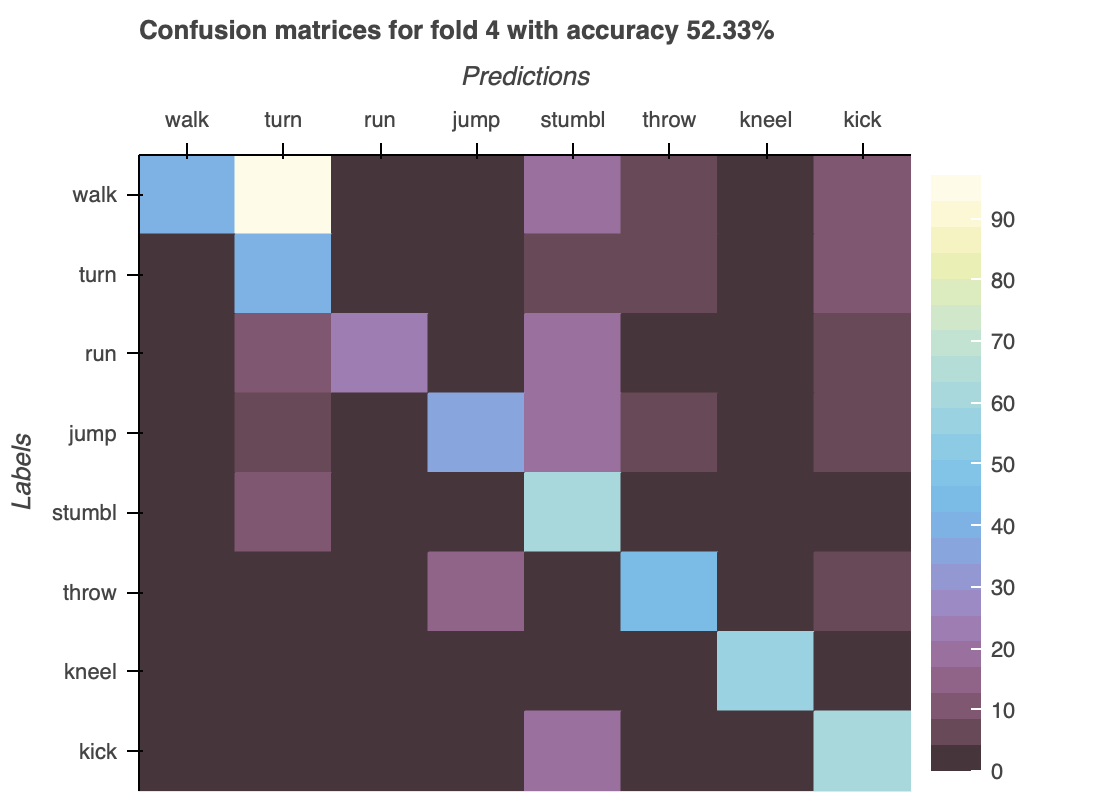
\includegraphics[width=\textwidth]{img/CNN-confusion_matrix.png}
				\caption{CNN}
			\end{subfigure}
			\hfill
			\begin{subfigure}[b]{0.49\textwidth}
				\centering
				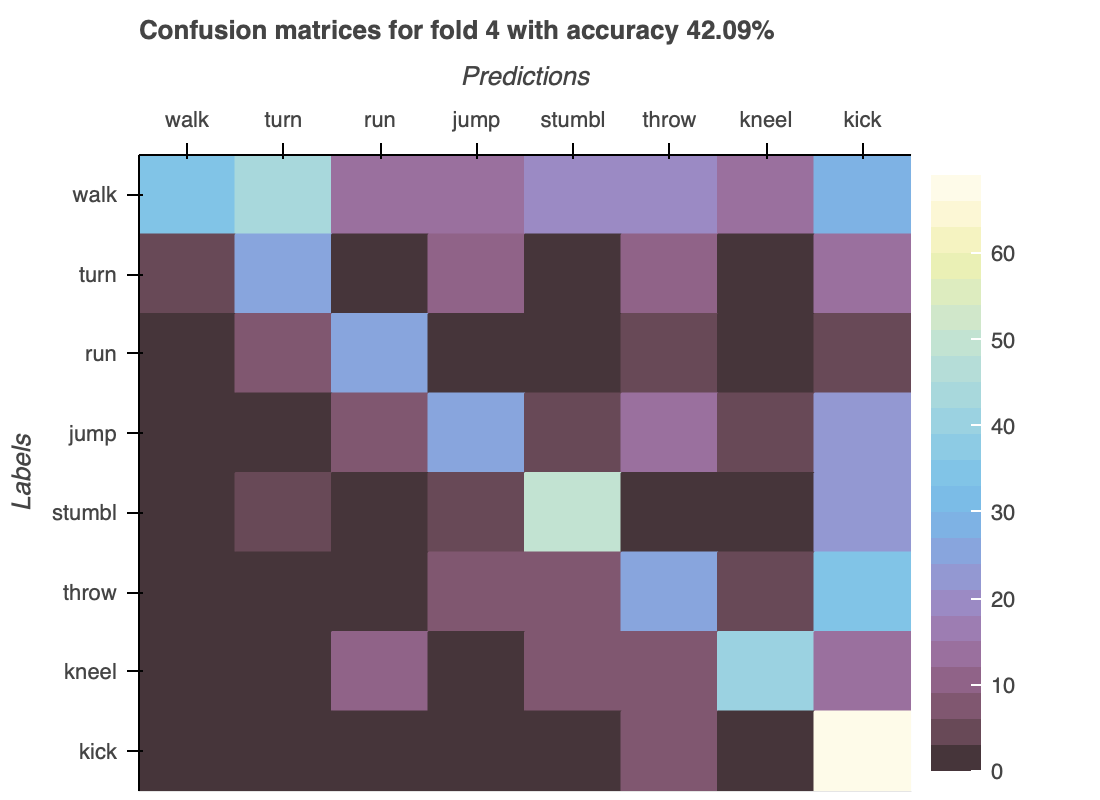
\includegraphics[width=\textwidth]{img/ResNet-confusion_matrix.png}
				\caption{ResNet}
			\end{subfigure}
			\caption{The best results achieved by one-to-one models}
			\label{fig:confusion-raw}
		\end{figure}
		However, using all the data available in the xml-file, i.e. the root joint position and rotation and the position of each joint, resulted in a decrease of the accuracy rates for all models. And show that adding more data didn't help much in making the trained models more robust. The issue behind this behaviour couldn't be overcome by the experimentation performed. However, the inherent problems with HAR, which differentiates it starkly from image recognition as an example, is intra-class similarity and inter-class variability, and makes finding good representations of human activities with more data a tedious endeavor. It is necessary to note that the accuracy rates achieved by the models using the all the data available in the xml-files aren't representative of the overall qualities of the models and must be viewed by the lenses of the associated confusion matrices. This is in part due to the unbalanced nature of the assembled dataset, and a model classifying all instances as the most dominant class is of less quality compared to a model having a less accuracy overall.\newline
		Plappert et al used a sampling frequency of 100 Hz, i.e. every 10 ms the state and shape of the body of the participant it taken\cite{Plappert2016}. This could make for the case that, the data extracted from the xml-file is very redundant, which would make dropping some of the frames and only considering a less dense representation of the motions very appealing. This approach would be very beneficial for reducing the complexity of training and thus the time needed for it. The visualization of the results of each experiment with reduced frequency show very little change in the accuracy and the behaviour of the loss function during training and validation. This makes this approach very promising for future works and experimentations.
		\begin{figure}[H]
			\centering
			\begin{subfigure}[b]{0.49\textwidth}
				\centering
				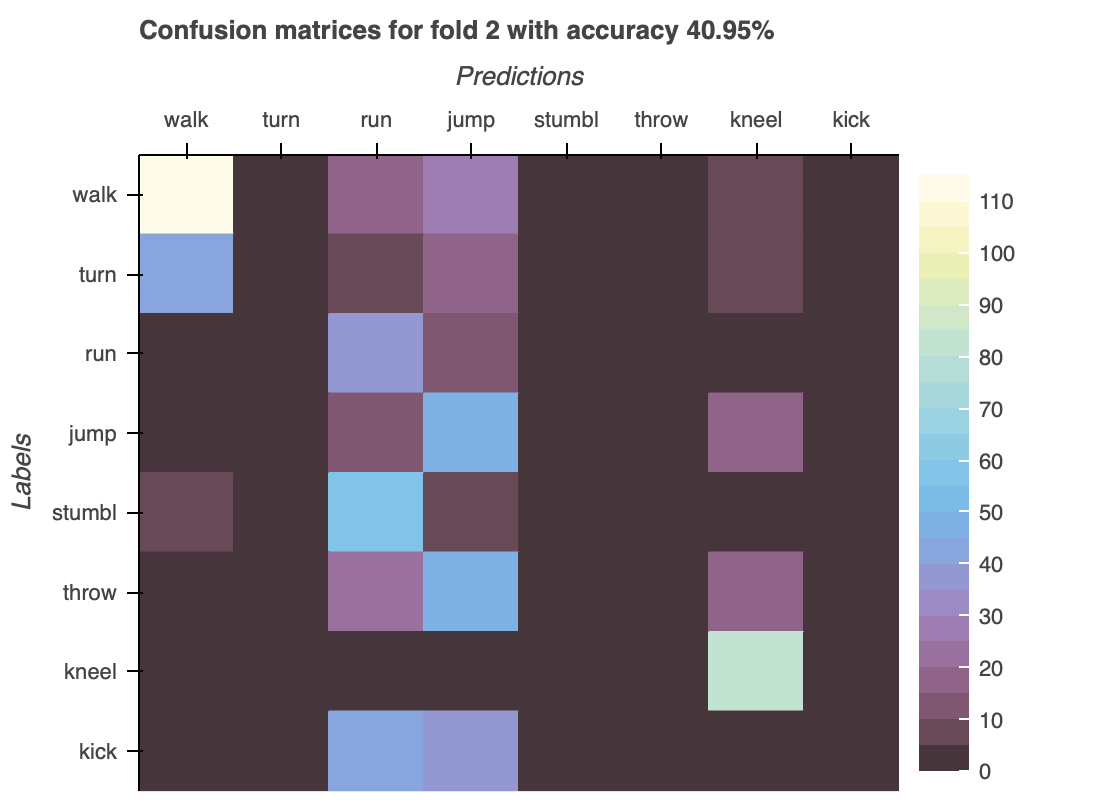
\includegraphics[width=\textwidth]{img/MLP-confusion_matrix_simplified.png}
				\caption{MLP}
			\end{subfigure}
			\hfill
			\begin{subfigure}[b]{0.49\textwidth}
				\centering
				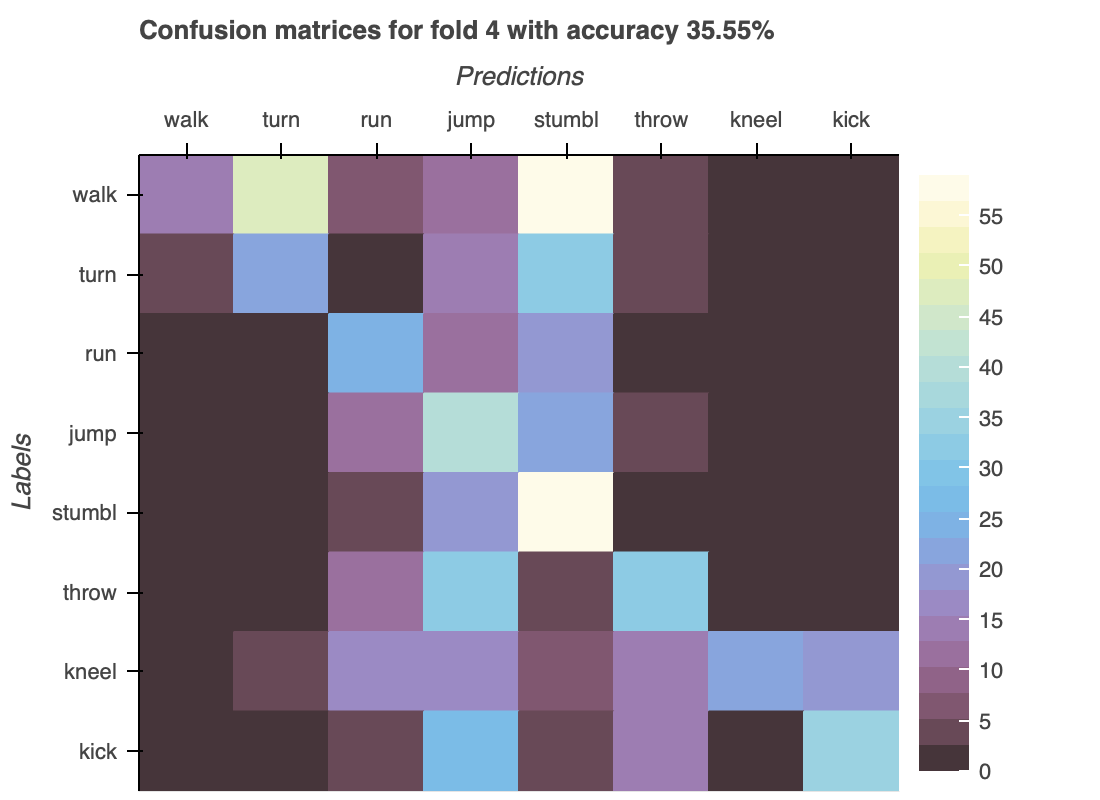
\includegraphics[width=\textwidth]{img/FCN-confusion_matrix_simplified.png}
				\caption{FCN}
			\end{subfigure}
			\hfill
			\begin{subfigure}[b]{0.49\textwidth}
				\centering
				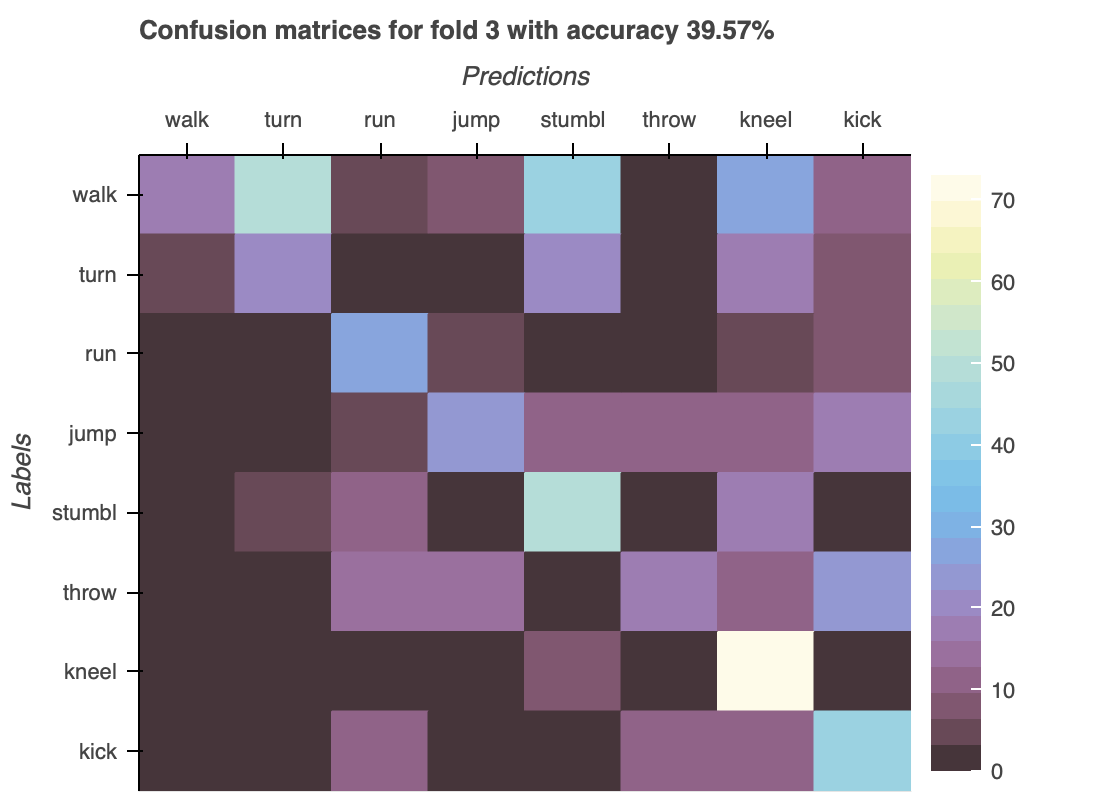
\includegraphics[width=\textwidth]{img/CNN-confusion_matrix_simplified.png}
				\caption{CNN}
			\end{subfigure}
			\hfill
			\begin{subfigure}[b]{0.49\textwidth}
				\centering
				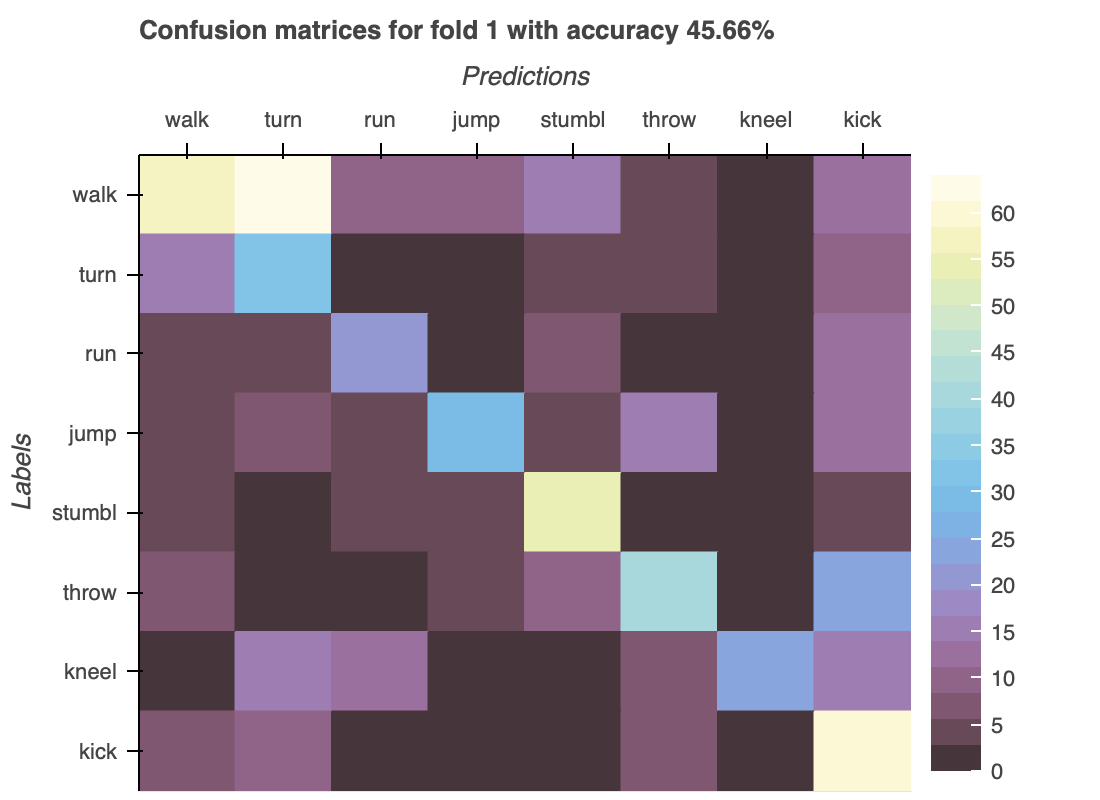
\includegraphics[width=\textwidth]{img/ResNet-confusion_matrix_simplified.png}
				\caption{ResNet}
			\end{subfigure}
			\caption{The confusion matrix achieved by using a frequency of 20 frames per seconds}
			\label{fig:freq_5}
		\end{figure}
	\section{Sequence-modelling learning machines}\label{subsec:eve_seq} 
		For this section the following learning machines will be used with each having 3 layers and a hidden size, i.e. the number of features in the hidden size, of 512:
		\begin{itemize}
			\item RNN and bi-RNN
			\item GRU and bi-GRU
			\item LSTM and bi-LSTM
		\end{itemize}
		Further experimentation for the hyper-parameters of the recurrent neural networks couldn't be done due to the time constraints and the prohibitive nature of training such models and the time necessary to complete them. In summery, these models offered less or no performance without using oversampling compared to learning machines in \ref{subsec:eva_one2one} and seem to perform poorly for all data, i.e. root information, joint position and the combination of both. This proves that these models are incompatible with the data extracted from the xml-files. As mentioned in the introductory part of this chapter. Training these models is very difficult and require a lot of resources, thus making the training with more epochs prohibitive and time-consuming. In addition to that during training they showed the same behavior with regard to the development of the loss values during training and validation. This is clearly demonstrable by fig \ref{fig:accuray_loss_seq_models}.
		\begin{figure}[H]
			\centering
			\begin{subfigure}[b]{0.49\textwidth}
				\centering
				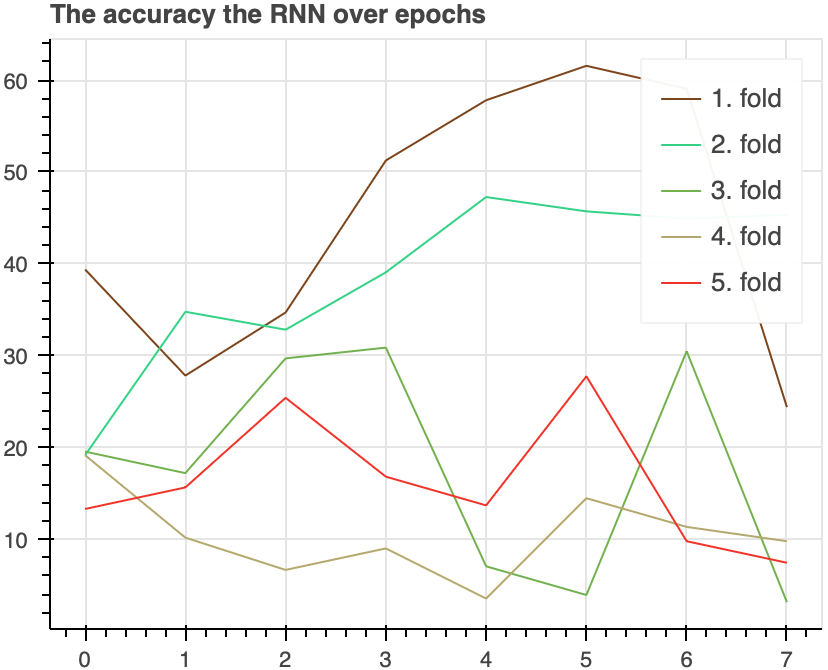
\includegraphics[width=\textwidth]{img/RNN-accuracy.png}
			\end{subfigure}
			\begin{subfigure}[b]{0.49\textwidth}
				\centering
				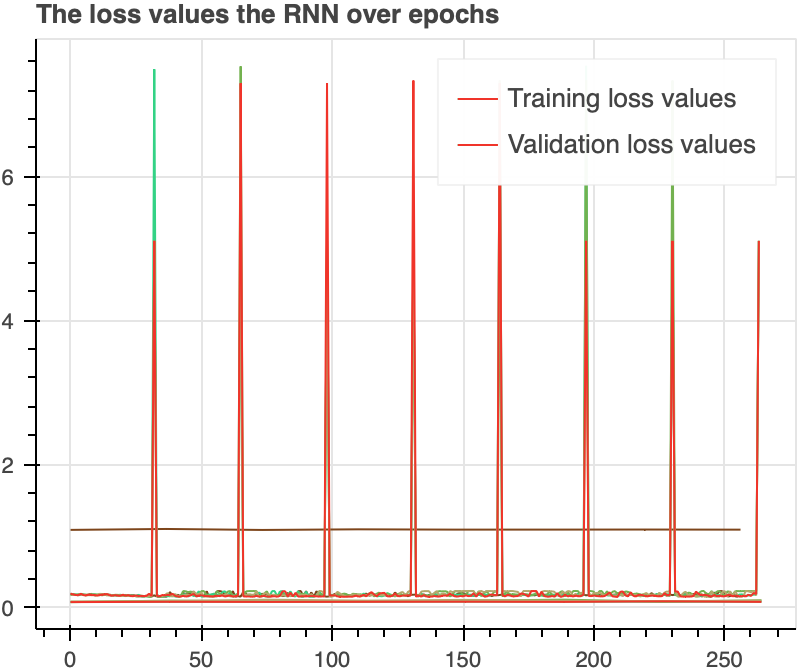
\includegraphics[width=\textwidth]{img/RNN-loss_values.png}
			\end{subfigure}
			\hfill
			\begin{subfigure}[b]{0.49\textwidth}
				\centering
				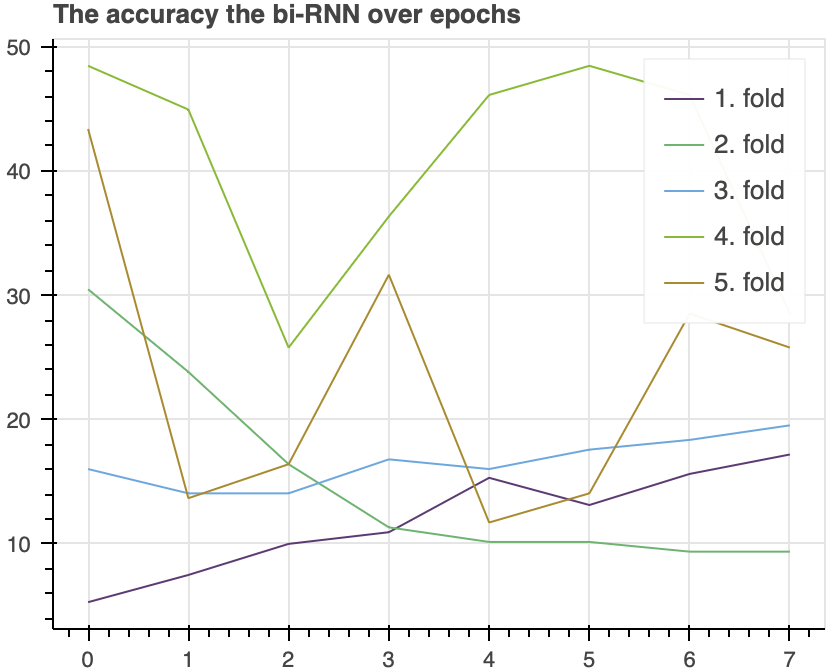
\includegraphics[width=\textwidth]{img/bi-RNN-accuracy.png}
			\end{subfigure}
			\begin{subfigure}[b]{0.49\textwidth}
				\centering
				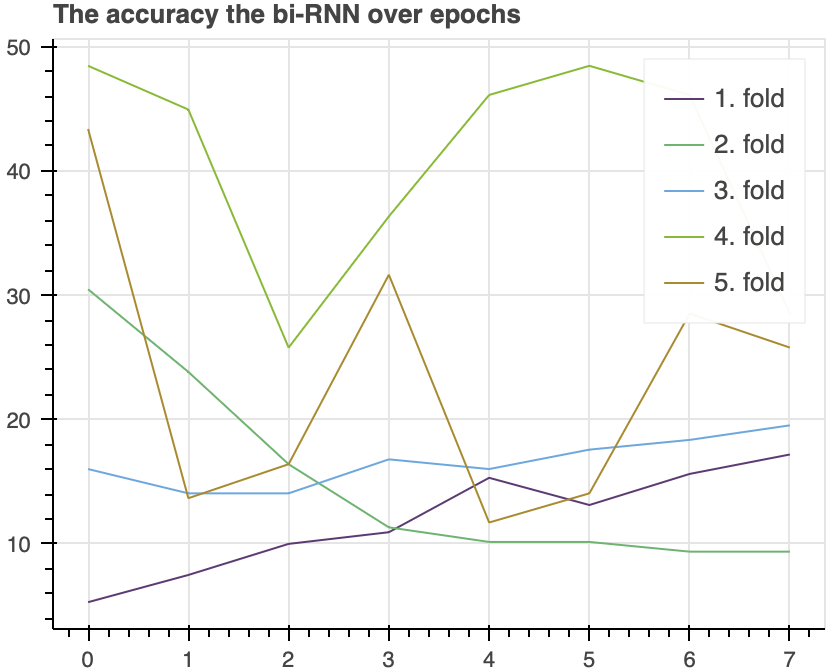
\includegraphics[width=\textwidth]{img/bi-RNN-loss_values.png}
			\end{subfigure}
			\hfill
			\begin{subfigure}[b]{0.49\textwidth}
				\centering
				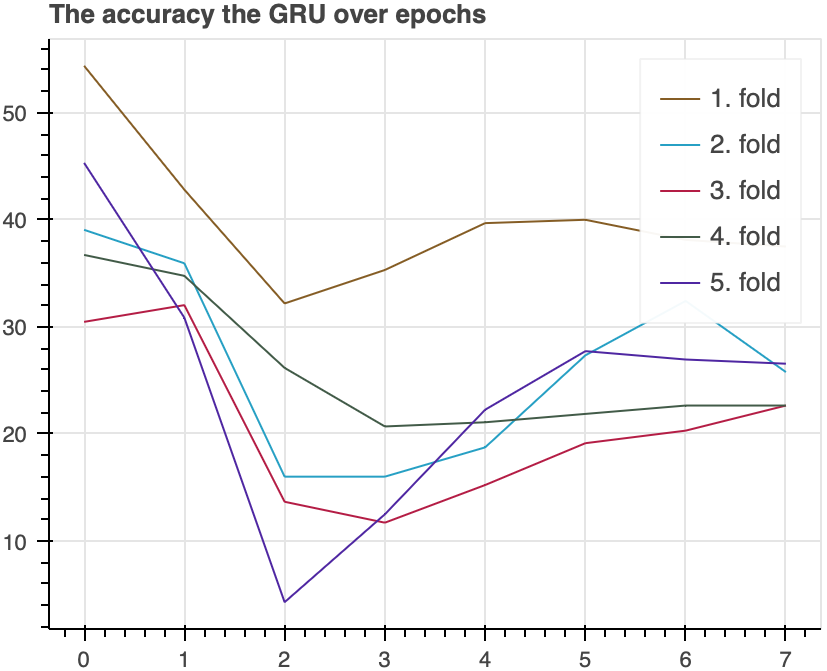
\includegraphics[width=\textwidth]{img/GRU-accuracy.png}
			\end{subfigure}
			\hfill
			\begin{subfigure}[b]{0.49\textwidth}
				\centering
				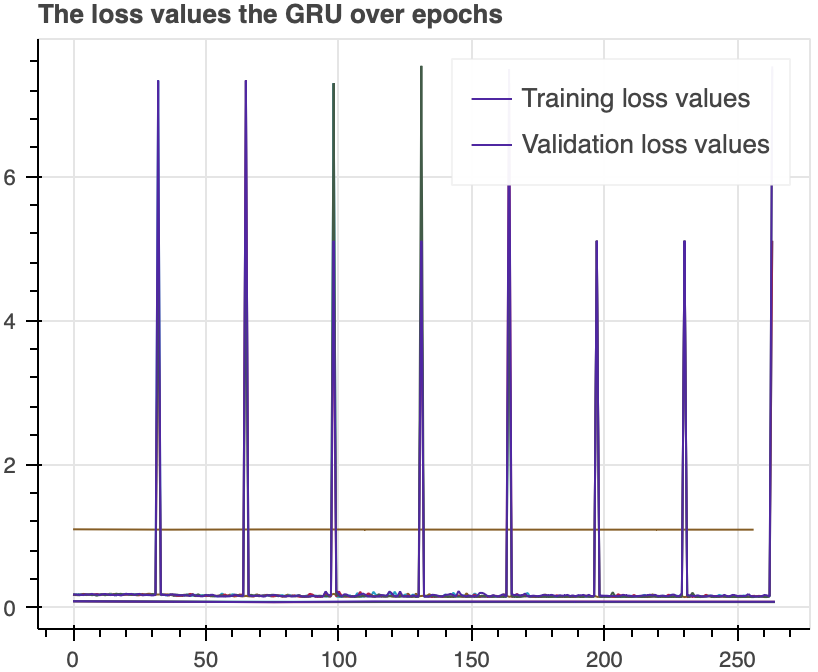
\includegraphics[width=\textwidth]{img/GRU-loss_values.png}
			\end{subfigure}
		\end{figure}
		\begin{figure}[H]\ContinuedFloat
			\begin{subfigure}[b]{0.49\textwidth}
				\centering
				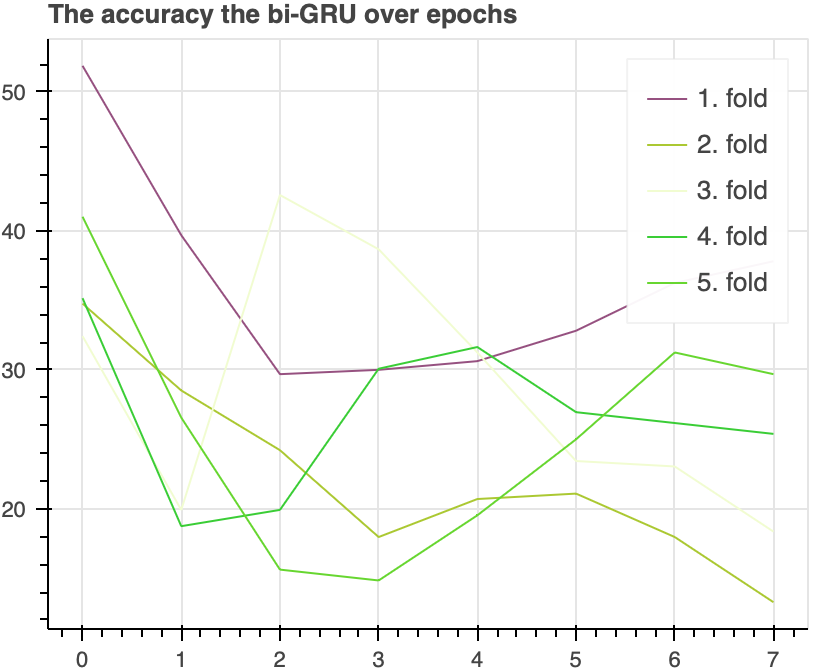
\includegraphics[width=\textwidth]{img/bi-GRU-accuracy.png}
			\end{subfigure}
			\hfill
			\begin{subfigure}[b]{0.49\textwidth}
				\centering
				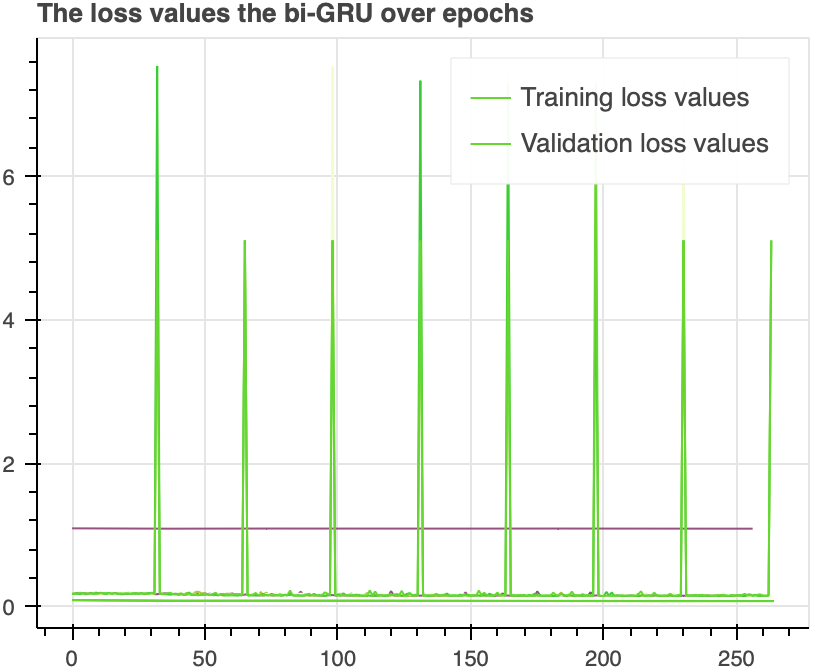
\includegraphics[width=\textwidth]{img/bi-GRU-loss_values.png}
			\end{subfigure}
		\end{figure}
		\begin{figure}[H]\ContinuedFloat
			\begin{subfigure}[b]{0.49\textwidth}
				\centering
				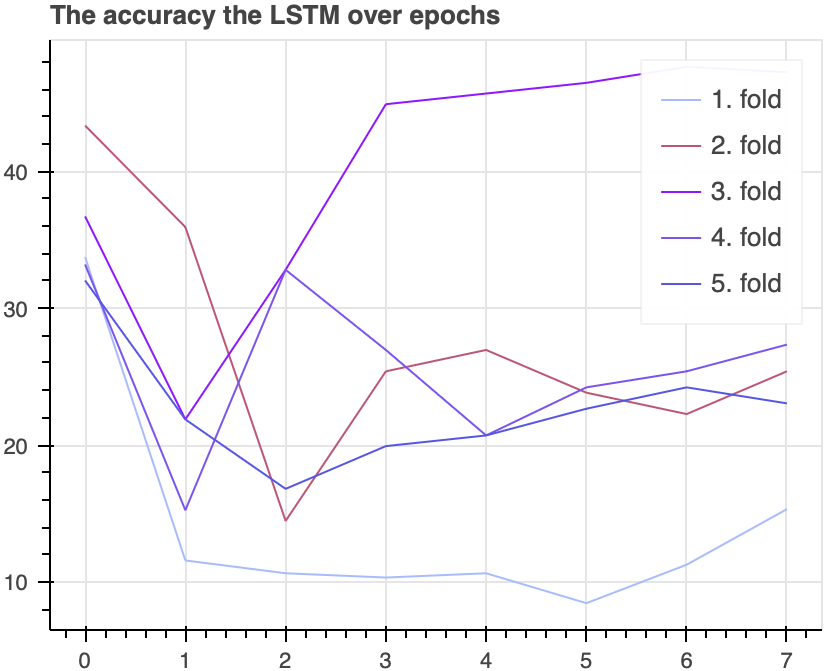
\includegraphics[width=\textwidth]{img/LSTM-accuracy.png}
			\end{subfigure}
			\hfill
			\begin{subfigure}[b]{0.49\textwidth}
				\centering
				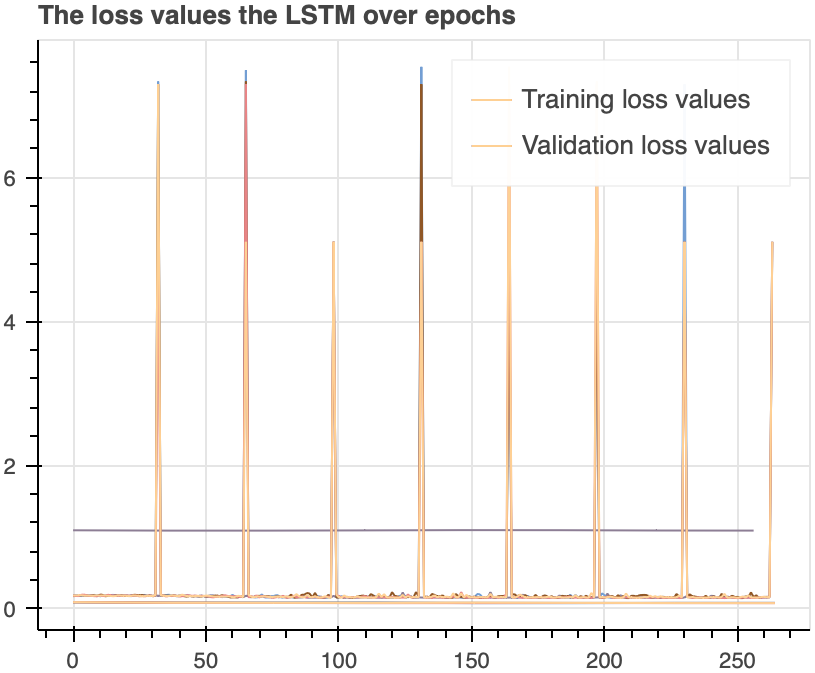
\includegraphics[width=\textwidth]{img/LSTM-loss_values.png}
			\end{subfigure}
			\hfill
			\begin{subfigure}[b]{0.49\textwidth}
				\centering
				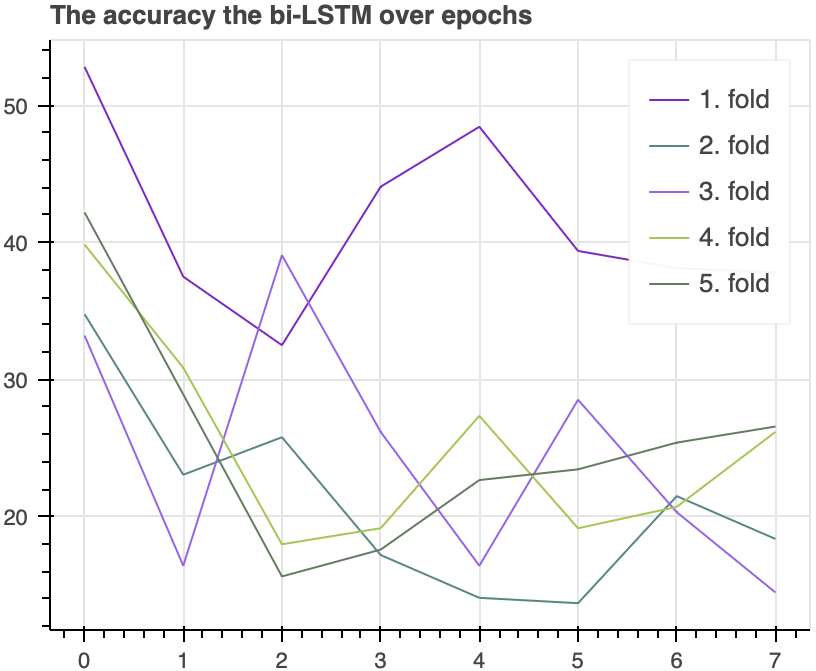
\includegraphics[width=\textwidth]{img/bi-LSTM-accuracy.png}
			\end{subfigure}
			\hfill
			\begin{subfigure}[b]{0.49\textwidth}
				\centering
				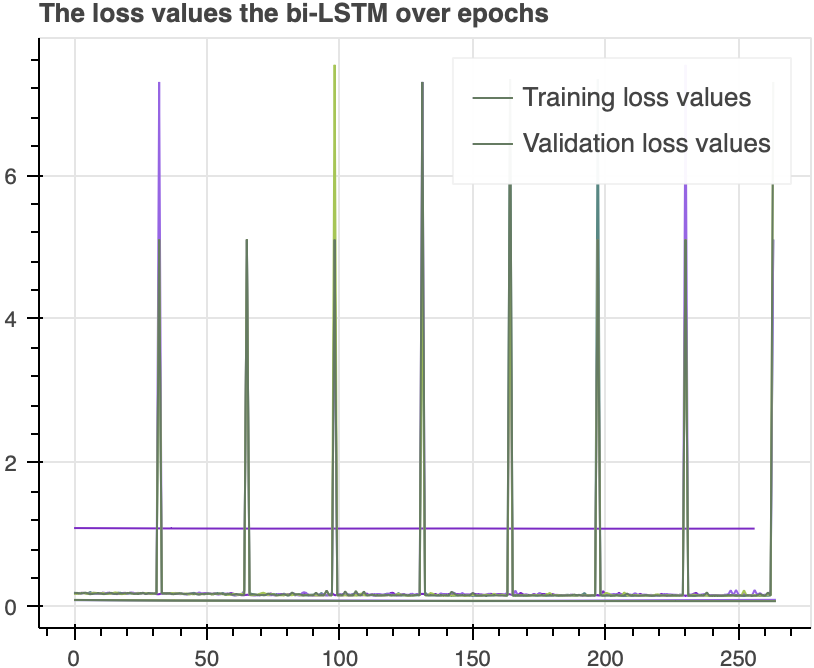
\includegraphics[width=\textwidth]{img/bi-LSTM-loss_values.png}
			\end{subfigure}
			\caption{The accuracy rate and the loss values over the epochs and during the training of sequence-modeling models}
			\label{fig:accuray_loss_seq_models}
		\end{figure}
		Using recurrent neural networks in this context with oversampling proved to be more robust than models in \ref{subsec:eva_one2one}, where the \textbf{walk} instances are correctly classified at a greater rate than one-to-one learning machines. This was the case for using all data extraction modes, as explained in the previous section. It must be noted that using only the root joint information lead to a greater results, as it can be easily noticed with the associated visualisation files. Nevertheless, bidirectional variants were less accurate and less robust and the accuracy rates achieved by them is very low despite the use of oversampling to their compared to their unidirectional counterparts. As for the recurrent neural networks variants themselves, RNNs proved to be the least performing and overcoming the hurdles of exploding/vanishing gradients and the other inherent problems mentioned in \ref{subsec:rnns} seem to bear fruits as both the bidirectional and unidirectional GRU and LSTM variants performed better than RNNs. This can be seen in fig \ref{fig:confusion-matrix-raw-seq}, where only the root joint information was used and oversampling was performed on the dataset. Nevertheless, these results are hugely contrasted by the results obtained with without oversampling with or without normalization, where recurrent neural networks performed worse on all fronts with an accuracy around 20\%. This is a huge indication that oversampling introduced overfitting to the model trained, even though theses accuracies where calculated on the validation dataset, as the model didn't see the instances in these sets for the first time during the validation process due to the duplication involved in oversampling. Lastly, experimenting with normalization proved produced the same results as in \ref{subsec:eva_one2one}, where it made the trained models less robust due to the nature of the information as explained in the previous section. Lastly, using all the data available in the xml-files only produced good results in combination with normalization, which makes a strong case for using it, if the data used is of varying nature, e.g. speed, velocity and position or with entirely different units of measure rad vs °.
		\begin{figure}[H]
			\centering
			\begin{subfigure}[b]{0.49\textwidth}
				\centering
				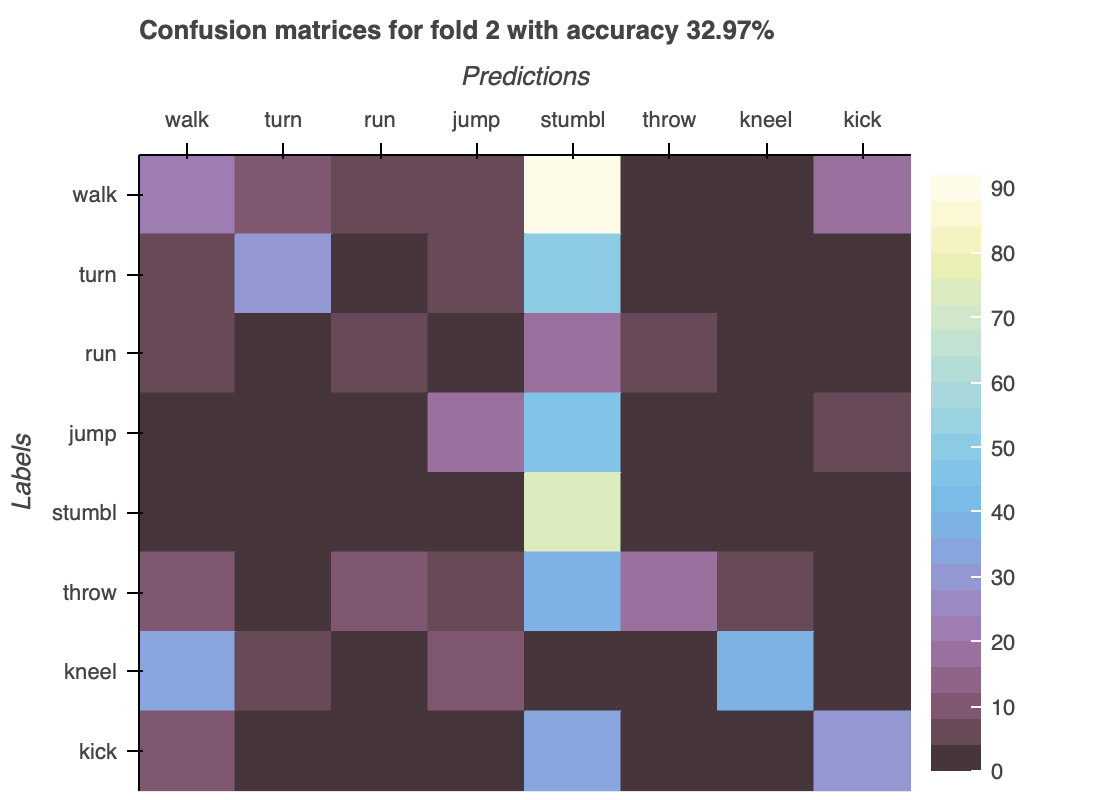
\includegraphics[width=\textwidth]{img/RNN-confusion_matrix.png}
				\caption{RNN}
			\end{subfigure}
			\hfill
			\begin{subfigure}[b]{0.49\textwidth}
				\centering
				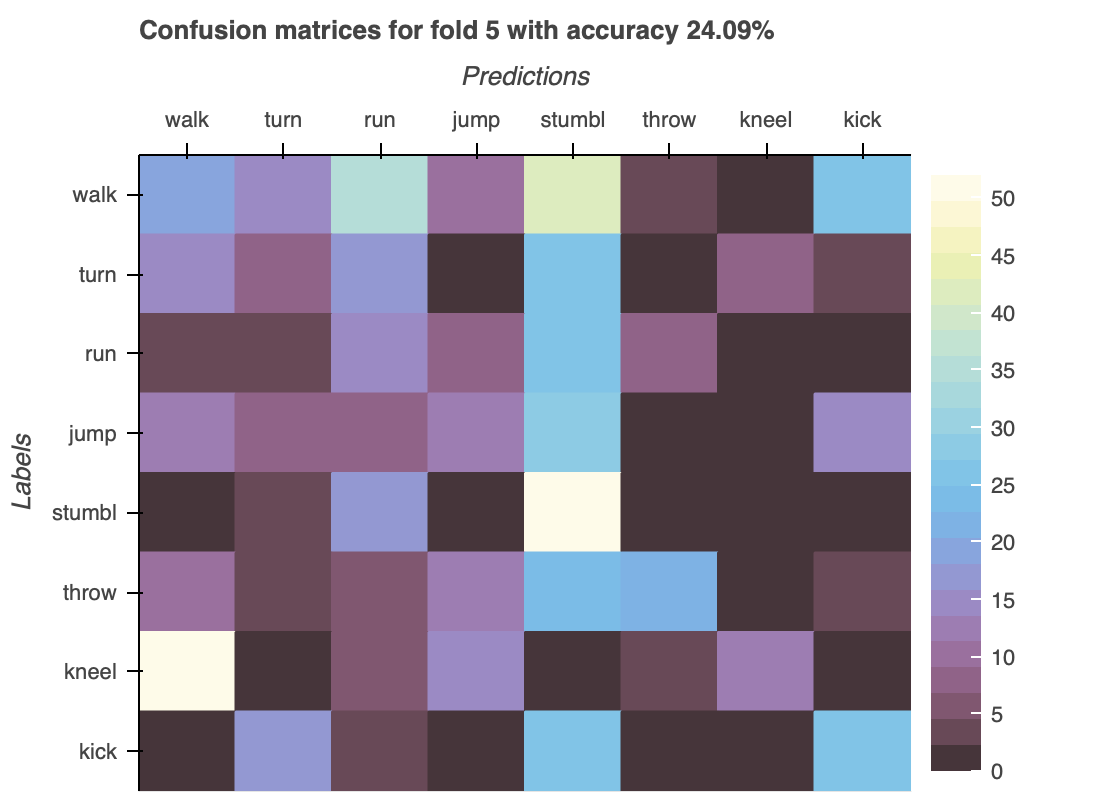
\includegraphics[width=\textwidth]{img/bi-RNN-confusion_matrix.png}
				\caption{bi-RNN}
			\end{subfigure}
			\hfill
			\begin{subfigure}[b]{0.49\textwidth}
				\centering
				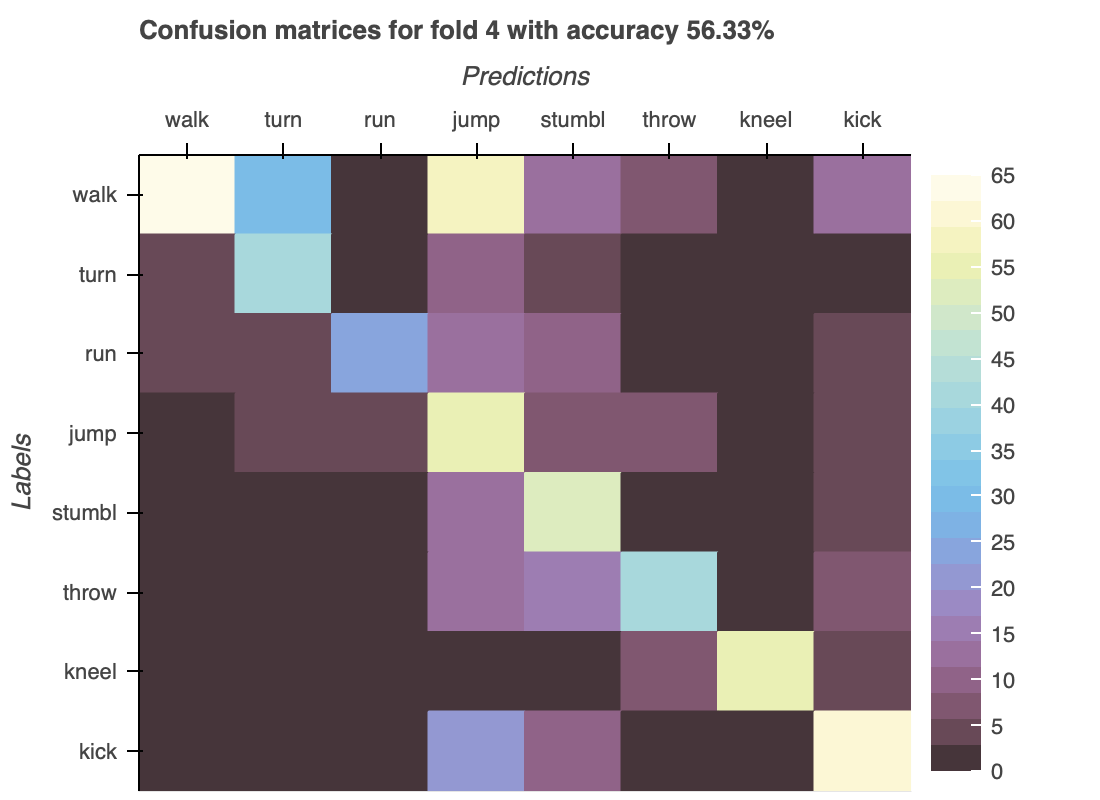
\includegraphics[width=\textwidth]{img/GRU-confusion_matrix.png}
				\caption{GRU}
			\end{subfigure}
			\hfill
			\begin{subfigure}[b]{0.49\textwidth}
				\centering
				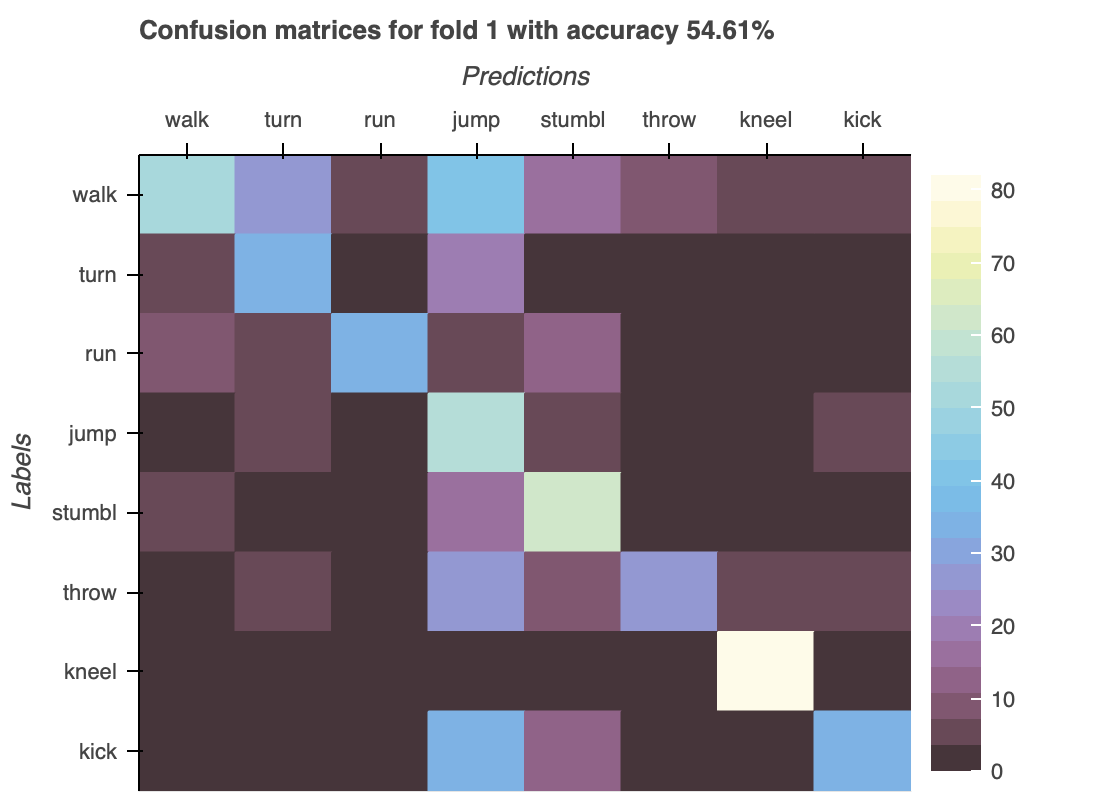
\includegraphics[width=\textwidth]{img/bi-GRU-confusion_matrix.png}
				\caption{bi-GRU}
			\end{subfigure}
			\hfill
			\begin{subfigure}[b]{0.49\textwidth}
				\centering
				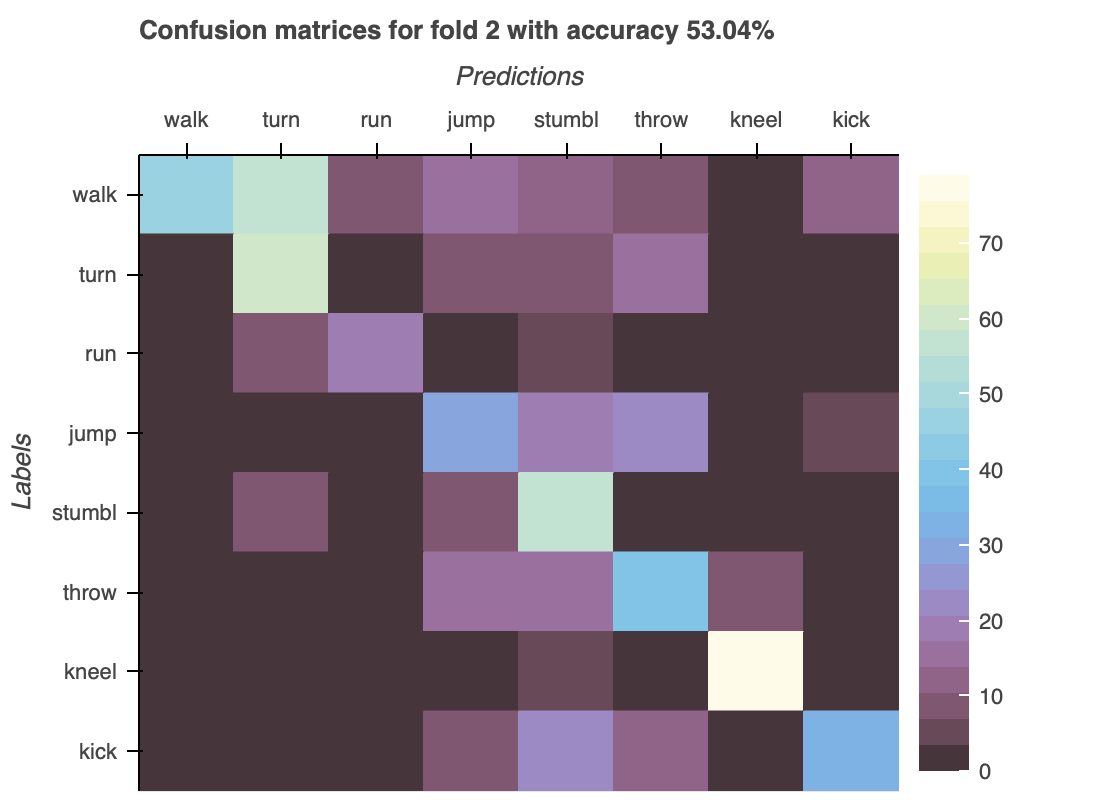
\includegraphics[width=\textwidth]{img/LSTM-confusion_matrix.png}
				\caption{LSTM}
			\end{subfigure}
			\hfill
			\begin{subfigure}[b]{0.49\textwidth}
				\centering
				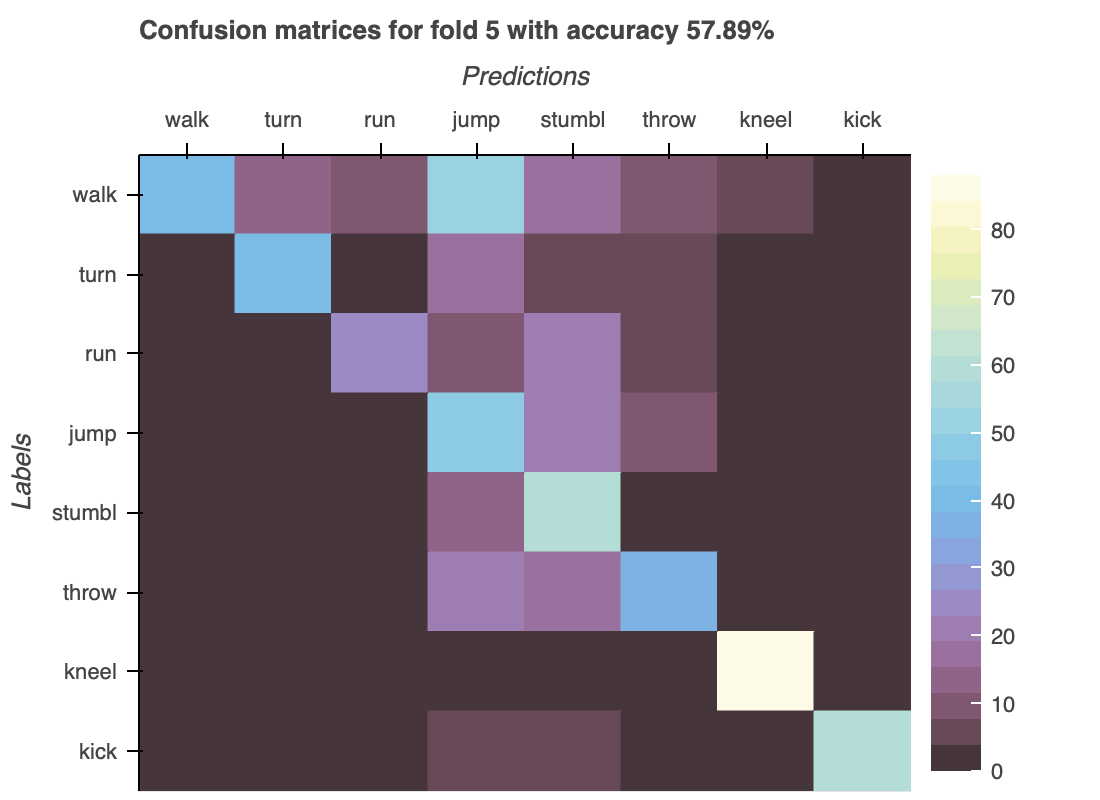
\includegraphics[width=\textwidth]{img/bi-LSTM-confusion_matrix.png}
				\caption{bi-LSTM}
			\end{subfigure}
			\caption{The best results achieved by RNNs and their variants}
			\label{fig:confusion-matrix-raw-seq}
		\end{figure}
		% TODO check if this hold for reduced frequency
		\newpage
		Just like \ref{subsec:eva_one2one} reducing the number of frames would be very beneficial, more so for machine learning algorithms that take longer to train on very long sequences, as it is the case for recurrent neural networks and their variants in this thesis. In addition to that, it has been documented in \ref{subsec:rnns} that these models don't perform well with problems having long-range temporal dependencies, thus making the reduction of frames doubly beneficial. The visualizations of the results obtained by training the models with reduced frequency show how the accuracy changed due to reducing the frequency of the frames in each motion for recurrent neural networks and their variants, where a serious deterioration of the performances metrics was ascertained. This makes this approach of simplification at a very high drop rate of frames ill-considered. The same can be said also about the bidirectional variants of recurrent neural networks, which performed generally worse than their unidirectional counterparts. Thus, it can be said with these results that the associated additional computational costs of using bi-directionality makes the use of bidirectional recurrent neural networks very unappealing in the context of HAR.
		\begin{figure}[H]
			\centering
			\begin{subfigure}[b]{0.49\textwidth}
				\centering
				\includegraphics[width=\textwidth]{img/RNN-confusion_matrix_drop.png}
				\caption{RNN}
			\end{subfigure}
			\hfill
			\begin{subfigure}[b]{0.49\textwidth}
				\centering
				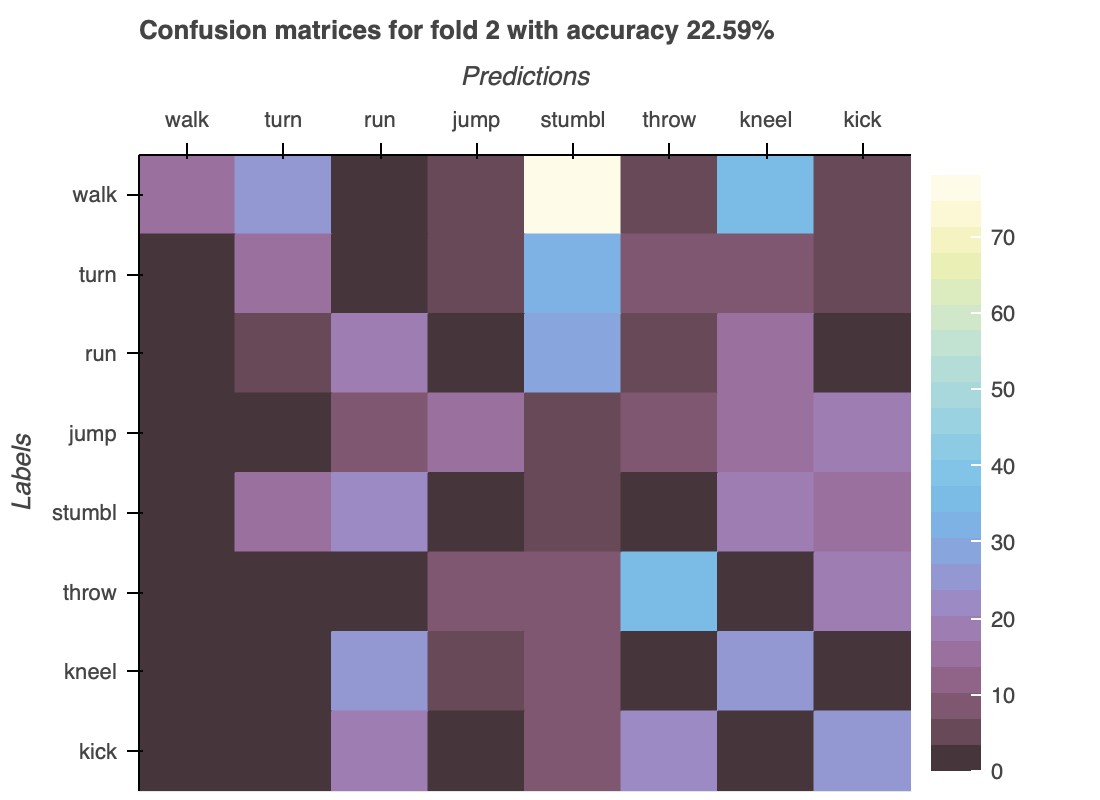
\includegraphics[width=\textwidth]{img/bi-RNN-Confusion_matrix_drop.png}
				\caption{bi-RNN}
			\end{subfigure}
		\end{figure}
		\begin{figure}[H]\ContinuedFloat
			\begin{subfigure}[b]{0.49\textwidth}
				\centering
				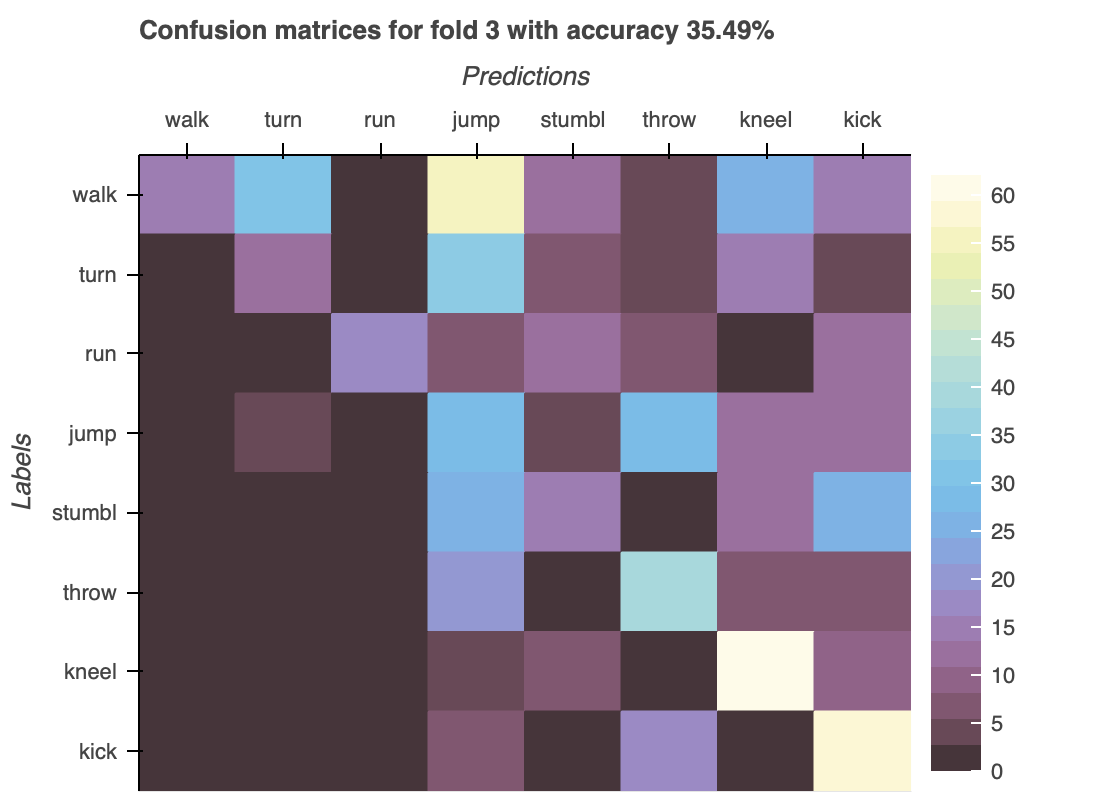
\includegraphics[width=\textwidth]{img/GRU-Confusion_matrix_drop.png}
				\caption{GRU}
			\end{subfigure}
			\hfill
			\begin{subfigure}[b]{0.49\textwidth}
				\centering
				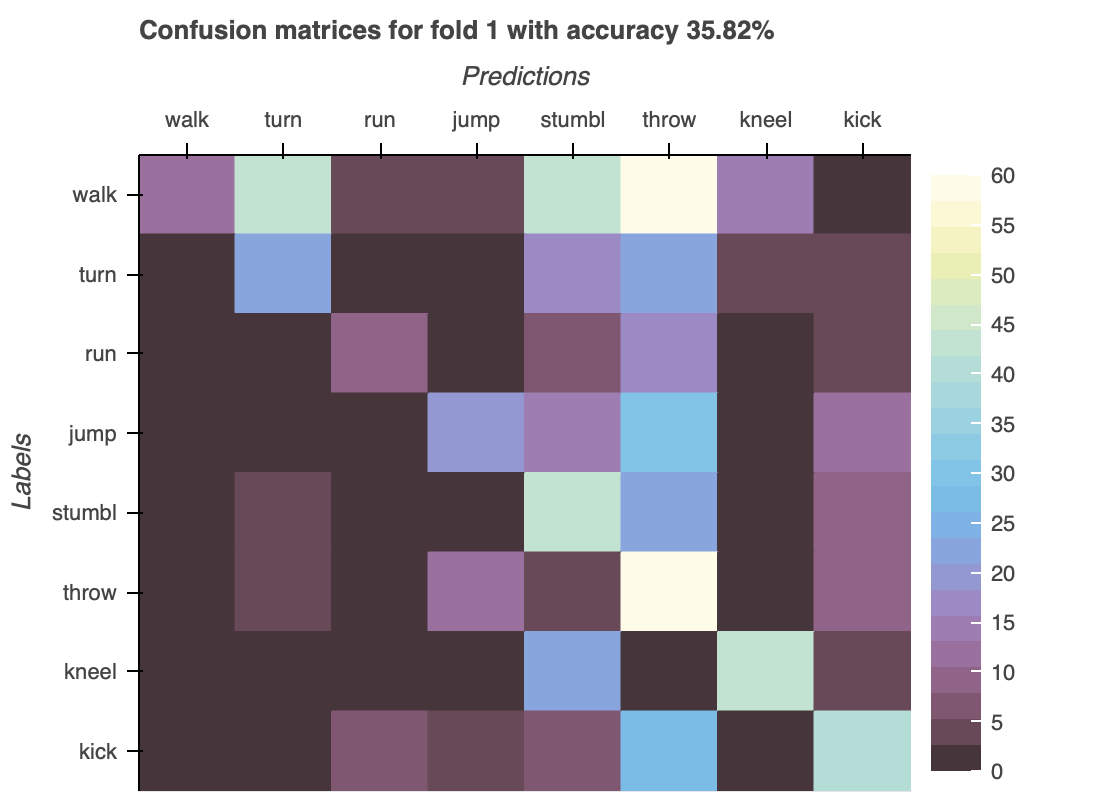
\includegraphics[width=\textwidth]{img/bi-GRU-Confusion_matrix_drop.png}
				\caption{bi-GRU}
			\end{subfigure}
			\begin{subfigure}[b]{0.49\textwidth}
				\centering
				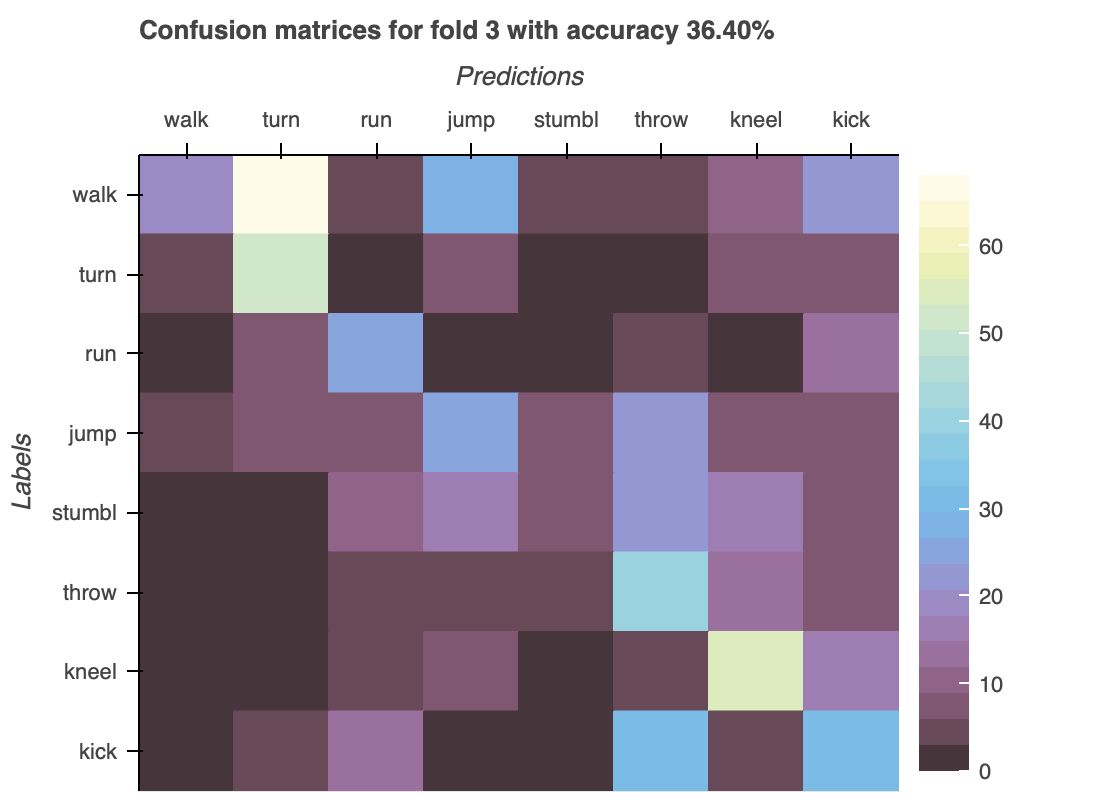
\includegraphics[width=\textwidth]{img/LSTM-Confusion_matrix_drop.png}
				\caption{LSTM}
			\end{subfigure}
			\hfill
			\begin{subfigure}[b]{0.49\textwidth}
				\centering
				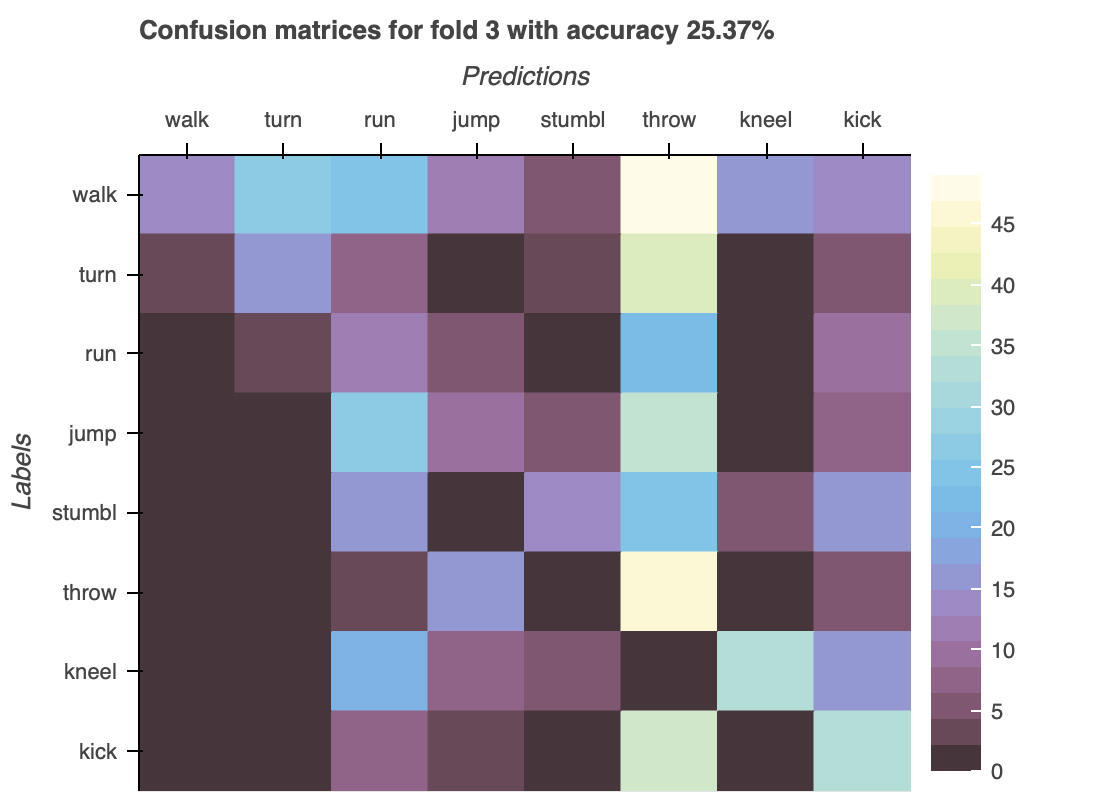
\includegraphics[width=\textwidth]{img/bi-LSTM-Confusion_matrix_drop.png}
				\caption{bi-LSTM}
			\end{subfigure}
			\caption{The confusion matrix achieved by using a frequency of 20 frames per seconds with recurrent neural networks in combination with oversampling and normalization}
			\label{fig:freq_5_seq}
		\end{figure}
